\documentclass[12pt,a4paper]{article}
\usepackage[utf8]{inputenc}
\usepackage[french]{babel}
\usepackage[T1]{fontenc}
\usepackage{amsmath}
\usepackage{amsfonts}
\usepackage{amssymb}
\usepackage{graphicx}
\usepackage{subcaption}
\usepackage{color}
\usepackage{fixltx2e} %math in title
\usepackage{algorithm}
\usepackage{algpseudocode}
\usepackage{placeins}
\usepackage{mvmsh}
\usepackage{frbib}
\usepackage[numbers]{natbib}

\bibliographystyle{abbrvnat-fr}

%\newcommand{\vecx}{\boldsymbol{x}}
%\newcommand{\vecxi}{\boldsymbol{\xi}}
%\newcommand{\vecdelta}{\boldsymbol{\delta}}
%\newcommand{\vecg}{\boldsymbol{g}}
%\newcommand{\vecn}{\boldsymbol{n}}
%
%\newcommand{\normT}[1]{\vecn_#1^T}
%
%\newcommand{\nabref}{\nabla_{\xi\eta}}
%\newcommand{\pxi}{\partial \xi}
%\newcommand{\peta}{\partial \eta}
%
%\newcommand{\phii}{\varphi_i}
%\newcommand{\phij}{\varphi_j}
%
%\newcommand{\dom}{\Omega}
%\newcommand{\domRef}{\Omega_{\vecxi}}
%\newcommand{\bordRef}{\partial \domRef}
%
%\newcommand{\iDom}[1]{\int_{\domRef}{#1 d\vecxi}}
%\newcommand{\iDomh}[1]{\int_{\domRef^h}{#1 d\vecxi}}
%\newcommand{\iBord}[1]{\int_{\bordRef}{#1 ds}}
%\newcommand{\iT}[1]{\int_{T}{#1 d\vecxi}}
%
%\newcommand{\Ks}{\tilde{K}}
%\newcommand{\Tt}{\tilde{T}}
%\newcommand{\To}{\overline{T}}
%\newcommand{\Nn}{N_{neig}}


\title{Rapport final du stage}
\author{Joao Guilherme CALDAS STEINSTRAESSER}

\begin{document}
  \maketitle
  \tableofcontents
  \section{Introduction}

\indent L'objectif de l'adaptation de maillages développée dans ce stage est de modifier la position de ses noeuds par rapport à une fonction donnée, ou à une solution d'un problème physique, de façon qu'on puisse avoir un raffinement variable au long du domaine et qui représente bien la présence de fortes gradients, surfaces, etc., sans modifier le nombre de points ni la connectivité du maillage.

\indent Dans ce rapport, on va présenter dans un premier moment l'application de l'algorithme à l'adaptation à des fonctions Level Set, à fin d'obtenir une bonne représentation d'un objet. Cette fonction, définie pour tout point du maillage, est la distance signée entre le point et l'objet, où la signe indique s'il est à son intérieur ou extérieur \cite{ducrot}. Ainsi, la ligne de niveau 0 de la fonction Level Set représente la surface de l'objet, et on utilisera ce fait pour orienter l'adaptation du maillage.

\indent Ensuite, on résoudra des problèmes de la mécanique des fluides sur les maillages adaptés et, avec les résultats obtenus, on fera des nouvelles adaptations, mais cette fois-ci en utilisant au même temps la fonction Level Set et la solution physique du problème. Avec cette procédure, on sera capable d'obtenir des maillages encore plus appropriées au calcul envisagé. 

\indent Le rapport est organisé de la façon suivante : dans la section \ref{sec:modele}, on va d'abord présenter, de façon plus générale, le modèle utilisé pour l'adaptation de maillages, selon la formulation développée par \cite{arpaia}, et des détails concernant son implémentation. L'application du modèle à l'adaptation à des fonctions Level Set sera décrite dans la section \ref{sec:application}, avec quelques exemples de tests réalisés et une indication des paramètres qui ont produit les meilleurs résultats. Le couplage avec l'adaptation physique et les résultats obtenus sont présentés dans la section \ref{sec:adapPhysique}. Enfin, dans la section \ref{sec:nonstat}, on utilise le modèle pour adapter le maillage à des objets en mouvement. Par ailleurs, on remarque que la plupart du contenu de ce rapport se réfère à des cas 2D; pourtant, nous présentons aussi quelques résultats pour des exemples 3D.

\indent Les exemples présentés dans ce rapport ne sont qu'une petite partie de l'ensemble des tests réalisées  au cours de ce stage. Ces tests ont eu une grande importance pour valider, corriger et développer le modèle,  tester la bibliothèque et les plusieurs parties du code, et trouver les paramètres et stratégies d'adaptation qui nous permettent d'obtenir les meilleurs résultats en tenant compte des objectifs décrits ci-dessus. La section \ref{sec:autres} présente une liste des rapports rédigées pour décrire et présenter ces tests.
  \section{Le modèle}
\label{sec:modele}

\subsection{Description du problème}

\indent On va faire la distinction entre deux domaines : 

\begin{itemize}
  \item \textbf{Domaine physique ou réel } (\(\vecx =(x,y)\)) : domaine déformable, noté \(\dom\);
  \item \textbf{Domaine computationnel ou de référence } (\(\vecxi =(\xi,\eta)\)) : domaine fixé, noté \(\domRef\)
\end{itemize}

\indent On cherche une fonction 

\begin{equation*}
  \vecx = \vecx(\vecxi)
\end{equation*}

\indent Dans le modèle utilisé, on va considérer que la position \(\vecx\) des noeuds du maillage est régie par l'équation

\begin{equation*}
  %\label{eq:laplacien}
  \nabref \cdot \left( \omega \nabref \vecx \right) = 0
\end{equation*}

\noindent où \(\nabref\) est le gradient par rapport aux coordonnées de référence et \(\omega\) est une fonction de \(\vecx\) qui contient l'information qui déterminera le mouvement des noeuds. Dans le travail développé au cours du stage, on a implémenté deux modèles différents pour le calcul de cette fonction : 

\begin{enumerate}
	\item Dans un première moment, on a implémenté utilisé dans \cite{arpaia} : en supposant qu'on fait l'adaptation par rapport à une fonction \(u\), \(\omega\) est donné par l'expression

	\begin{equation*}
  		\omega(\vecx) = \sqrt{1 + \alpha ||\nabref u(\vecx)|| + \beta ||H(u)(\vecx)||}
	\end{equation*}

	\indent \(H(u)\) est le hessien de \(u\), et \(\alpha\) et \(\beta\) sont des paramètres choisis par l'utilisateur. Pour que ce choix soit moins dépendant du problème, on va toujours considérer les gradients et le hessiens normalisés.
	
	\item On a ensuite utilisé un modèle où on fournit directement à chaque noeud \(i\) la taille de maille \(\hdes\) qu'on désire, selon la formulation présentée par \cite{askes} : 
	
	\begin{equation}
		\label{eq:omega2}
		\omega(\vecx) = \frac{1}{\hdes(\vecx)}
	\end{equation}
	
	\indent La façon dont on calcule les tailles désirées dépende du type d'adaptation qu'on fait (adaptation à une fonction Level Set ou à une solution physique), comme on précisera dans les sections suivantes de ce rapport.
	
	
\end{enumerate} 

\indent Pour que le problème soit bien posé, il faut définir des conditions aux bords appropriées : 

\begin{equation}
	\label{eq:systeme}
	\begin{cases}
  		\nabref \cdot \left( \omega \nabref \vecx \right) = 0 \ \ dans \ \ \domRef \\
  		\vecx = \vecg \ \ sur \ \ \bordRef^D \\
  		\nabref \vecx \cdot \vecn = 0 \ \ sur \ \ \bordRef^N 
	\end{cases}
\end{equation}

\indent Ainsi, les conditions aux limites utilisées sont de deux types, de Dirichlet et de Neumann, définies sur des parties disjointes du bord, (\(\bordRef^D\) et \(\bordRef^N\), respectivement). Pour les conditions de Dirichlet, on impose \(\vecg = \vecxi\), indiquant que les points de \(\bordRef^D\) ne doivent pas bouger (ce qu'on impose, par exemple, dans les coins d'un domaine rectangulaire). En revanche, les conditions de Neumann (imposées par exemple dans les côtés du domaine), indiquent que les points de \(\bordRef^N\) doivent glisser sur le bord, i.e., bouger parallèlement  au bord (de façon que, dans notre exemple, le domaine reste toujours rectangulaire).

\indent La formulation faible du problème, avec une fonction test  \(v \in H_1^0(\domRef)\), s'écrit comme

\begin{equation}
	\label{eq:faible}
	0 = \iDom{v\nabref \cdot \left( \omega \nabref \vecx \right)} = -\iDom{\omega \nabref v \cdot \nabref \vecx} + \iBord{v\omega\nabref \vecx \cdot \vecn} 
\end{equation}

\indent Les conditions aux bords définies en \eqref{eq:systeme} annulent le dernier terme en \eqref{eq:faible}, et on arrive ainsi à 

\begin{equation*}
	\iDom{\omega \nabref v \cdot \nabref \vecx} = 0
\end{equation*}




\subsection{Discrétisation en éléments finis}

\indent On utilise une discrétisation en élément finis P1, avec une base de fonctions \(\{\phii\}\) définis pour chacun des \(N\) noeuds du maillage. Ainsi, \(\vecx\) et la fonction test \(v \in H_0^1(\dom)\) se discrétisent sous la forme

\begin{equation}
  \label{eq:u_disc}
  \begin{gathered}
  \vecx_h = \sum_{j=1}^N{\vecx_j\phij} = \sum_{j=1}^N{ \left( \begin{array}{c}  x_j \\ y_j \end{array} \right)    \phij} \\
  v_h = \sum_{i=1}^N{v_i\phii} 
  \end{gathered}
\end{equation}

\indent En utilisant \eqref{eq:u_disc} dans \eqref{eq:faible}, on arrive à

\begin{equation*}
	\sum_{j=1}^N{ \left[  \left( \iDomh{ \omega \nabref \phii \cdot \nabref \phij }  \right)  \vecx_j \right] } = 0 \ \ \forall i \in \{1,...,N\}
\end{equation*}

\indent On voit ainsi que la discrétisation en éléments finis se ramène à la résolution de deux systèmes linéaires indépendants et de la même forme, un pour les coefficients \(\{x_j\}\) et l'autre pour \(\{y_j\}\) : 

\begin{equation}
	\label{eq:syst_final}
	\begin{cases}
		Kx = 0 \\
		Ky = 0
	\end{cases}
\end{equation}

\indent Les éléments de la matrice \(K\) ont la forme

\begin{equation}
  k_{ij} = \iDomh{ \omega \nabref \phii \cdot \nabref \phij }
\end{equation}


\subsection{Quelques éléments pour le calcul de \(K\)}
\label{subsec:calculK}

\indent Le calcul des éléments de K est fait de la manière usuelle, par assemblage des contributions des éléments pour les coefficients \(k_{ij}\). On précise dans la liste suivante quelques détails de l'implémentation de ce calcul : 

\begin{itemize}
	\item Le gradient de \(\phii\) sur l'élément \(T\) sera donnée par \((\nabref \phii)^T = \frac{\normT{i}}{d!|T|}\), où \(|T|\) est l'aire de \(T\), \(d=2\) est le nombre de dimensions spatiales et \(\normT{i}\) est le vecteur entrant à \(T\), dans le côté opposé à \(i\) et de norme égale à la longueur de ce côté \cite{vecNormal}.
	\item La fonction \(\omega\) sera considérée constante dans chaque élément \(T\) et égale à la moyenne \(\omega^T\) de sa valeur sur les noeuds de \(T\).
	\item Comme l'intégrale est calculée dans le domaine de référence, on utilisera toujours les vecteurs normaux et les aires du maillage initial. La fonction \(\omega\), en revanche, sera actualisée pour exprimer l'évolution du maillage, et son calcul sera faite en utilisant la solution interpolée à la fin de chaque itération.
\end{itemize}

\indent On a, ainsi : 

\begin{equation}
\label{eq:calculK_2d}
\begin{gathered}
\begin{aligned}
	k_{ij} & = \iDomh{ \omega \nabref \phii  \cdot \nabref \phij } = \sum_{T \ni i} {\iT{ \omega \nabref \phii \cdot \nabref \phij }} = \\
	       &  = \sum_{T \ni i}
	              { 
	                     { |T|\omega^T \frac{\normT{i}\cdot \normT{j}}{4|T|^2}
	                     }
	              }
	          = \sum_{T \ni i}
	              { 
	                     { \omega^T \frac{\normT{i}\cdot \normT{j}}{4|T|}
	                     }
	              }	              
\end{aligned}
\end{gathered}
\end{equation}

\indent \textbf{Remarque 1} : comme montre le développement du modèle fait ci-dessus, le calcul de l'intégrale qui donne les éléments de la matrice \(K\) est faite \textbf{toujours sur le maillage de référence}, ce qui implique que, dans \eqref{eq:calculK_2d}, on utilisera toujours les mêmes vecteurs normaux et les mêmes aires pour le calcul discret. Néanmoins, \textbf{la fonction \(\omega\) est actualisée à chaque itération dans le maillage physique}, afin de bien indiquer que, dans ses nouvelles positions, les nœuds sont dans des régions de raffinement ou pas.

\indent

\indent \textbf{Remarque 2} : Pour le calcul des éléments de \(K\), on a profité du fait que, dans la méthode d'éléments finis P1, on a \(k_{ij} = 0\) si les noeuds \(i\) et \(j\) n'appartient pas au même élément. Ainsi, la matrice est creuse, ce que nous a motivé à le stocker avec une structure adaptée (au lieu d'allouer une matrice de taille \(N \times N\)), afin de réduire la consommation d'espace mémoire, comme décrit ci-dessous : 


\begin{itemize}
	\item On identifie, d'abord, le nombre maximal de voisins d'un noeud du maillage, \(\Nn\), sous la convention qu'un noeud est toujours voisin de lui-même;
	\item On alloue deux vecteurs :  
	\begin{itemize}
		\item Un vecteur d'entiers, \(A\), de taille \((\Nn+1).(N+1)\);
		\item Un vecteur de doubles, \(\Ks\) , de taille \(\Nn.(N+1)\);
	\end{itemize}
%	\item Les éléments de ces vecteurs qui se réfèrent à l'élément \(i\) sont : 
%	\begin{itemize}
%		\item Dans \(A\) : \(A_{(\Nn+1).i}\) jusqu'à \(A_{(\Nn+1).(i+1)-1}\);
%		\item Dans \(\Ks\) : \(\Ks_{\Nn . i}\) jusqu'à \(\Ks_{\Nn  .(i+1)-1}\);
%	\end{itemize}
	\item Le vecteur \(A\) contient les index des voisins de chaque noeud. Par convention,
	\begin{itemize}
		\item \(A_{(\Nn+1).i} = \Nn^i\) contient le nombre de voisins de \(i\);
		\item \(A_{(\Nn+1).i+1}\) jusqu'à \(A_{(\Nn+1).i+\Nn^i}\) contiennent les index des voisins de \(i\) (pour commodité, on garde toujours \(A_{(\Nn+1).i+\Nn^i} = i\), mais cela n'est pas nécessaire)
	\end{itemize}
	\item Le vecteur \(\Ks\) contient les éléments de la matrice : 
	\begin{itemize}
		\item Si \(A_{(\Nn+1).i + z} = j\), alors \(\Ks_{\Nn . i + z - 1} = K_{ij}\)
	\end{itemize}
\end{itemize}

\indent Le stockage ici proposé n'est pas optimal, car, dans des maillages non structurés, les noeuds n'ont pas tous le même nombre de voisins. Par ailleurs, les \(\Nn+1\) premier éléments de \(A\) et les \(\Nn\) premiers éléments de \(\Ks\) ne sont pas utilisés, pour être en concordance avec les conventions d'index utilisés dans la bibliothèque MMG. Néanmoins, par rapport au stockage de la matrice complète, on a vérifié des très grandes avantages : 

\begin{itemize}
	\item Par exemple, dans un test avec environ \(28000\) noeuds et 165 mille élements non nulles dans la matrice \(K\), on est passé d'un stockage de 783 million de doubles (soit 0.02\% d'utilisation) à un stockage de 308 mille doubles (soit 54\% d'utilisation) et 336 mille entiers, avec un considérable gain en temps d'exécution.
	\item On a observé aussi des gains en temps d'exécution du programme. Dans la formulation originale, sans garder les index des voisins de chaque noeud, il fallait appeler une fonction qui retourne la liste de voisins. Cet appel était fait une fois par itération pour chaque noeud, lors de la résolution du système linéaire.
\end{itemize}


\subsection{Résolution du système linéaire}
\label{subsec:jacobi}

\indent Le système linéaire \eqref{eq:syst_final} est résolu de façon itérative, avec la méthode de Jacobi. Dans les tests, on utilise en général un nombre petit d'itérations (dix ou vingt), ce qui donne des bons résultats pour un temps de calcul raisonnable. La solution est calculée en terme des déplacements \(\vecdelta = \vecx - \vecxi\). Ainsi, on réécrit le système linéaire \eqref{eq:syst_final} sous la forme 

\begin{equation*}
	Kx = K(x-\delta+\delta) = 0 \longrightarrow K\delta = -K\xi
\end{equation*}

\indent où \(\vecdelta = \vecx - \vecxi\) est le déplacement des points. Ainsi, \(\forall i \in \{1,...,N\} \) :

\begin{equation*}
	k_{ii}\delta_i^{[n+1]} = -\sum_{j=1,j \neq i}^N k_{ij}\delta_{j}^{[n]} - \sum_{j=1}^N k_{ij}\xi_{j} = -\sum_{j=1}^N k_{ij}(\xi_j + \delta_{j}^{[n]}) + k_{ii}\delta_i^{[n]}
\end{equation*}

\indent Donc, finalement,

\begin{equation*}
	\delta_i^{[n+1]} =  \delta_i^{[n]} -\frac{1}{k_{ii}} \sum_{j=1}^N k_{ij}(x_j^{[n]})
\end{equation*}

\indent \textbf{Remarque} : avant d'actualiser la position des points, il faut vérifier si le déplacement calculé ne conduit pas à un croisement des noeuds. Pour faire cette vérification, on calculé les aires signés des éléments (i.e., en considérant l'ordre des noeuds). Si nécessaire, on relaxe le déplacement : 

%\begin{equation}
%	x_i^{[n+1]} = \xi_i + \theta \delta_i^{[n+1]}
%\end{equation} 

\begin{equation*}
	\vecx^{[n+1]} = \vecx^{[n]} + \theta \left( \vecxi + \vecdelta^{[n+1]} - \vecx^{[n]} \right)
\end{equation*} 

\noindent avec \(\theta \in [0,1]\). La relaxation est ainsi appliquée sur la différence entre deux positions successives, non pas sur le déplacement par rapport à la position initiale, car dans ce cas-ci on peut avoir de "retours en arrière" des points du maillage.
  \section{Application à la fonction Level Set}


\label{sec:application}

\indent Le modèle décrit dans la section précédente sera utilisé pour adapter le maillage par rapport à une fonction Level Set (LS). Cette fonction définit une distance signée entre chaque point du maillage et la surface qu'on représente: si le point \(\vecx\) est à l'extérieur de la surface, \(LS(\vecx) > 0\); s'il est à l'intérieur, \(LS(\vecx) < 0\); et si il est sur l'interface, \(LS(\vecx) = 0\).  On cherche alors à bouger les points pour avoir une meilleure représentation de la ligne de niveau 0 de la fonction Level Set, i.e., de la surface de l'objet \cite{ducrot}. Pour illustrer notre objectif, on présente dans la figure \ref{fig:exLS} un exemple d'adaptation à une fonction Level Set :

\begingroup
	\begin{minipage}[t]{.5\linewidth}
		\centering
		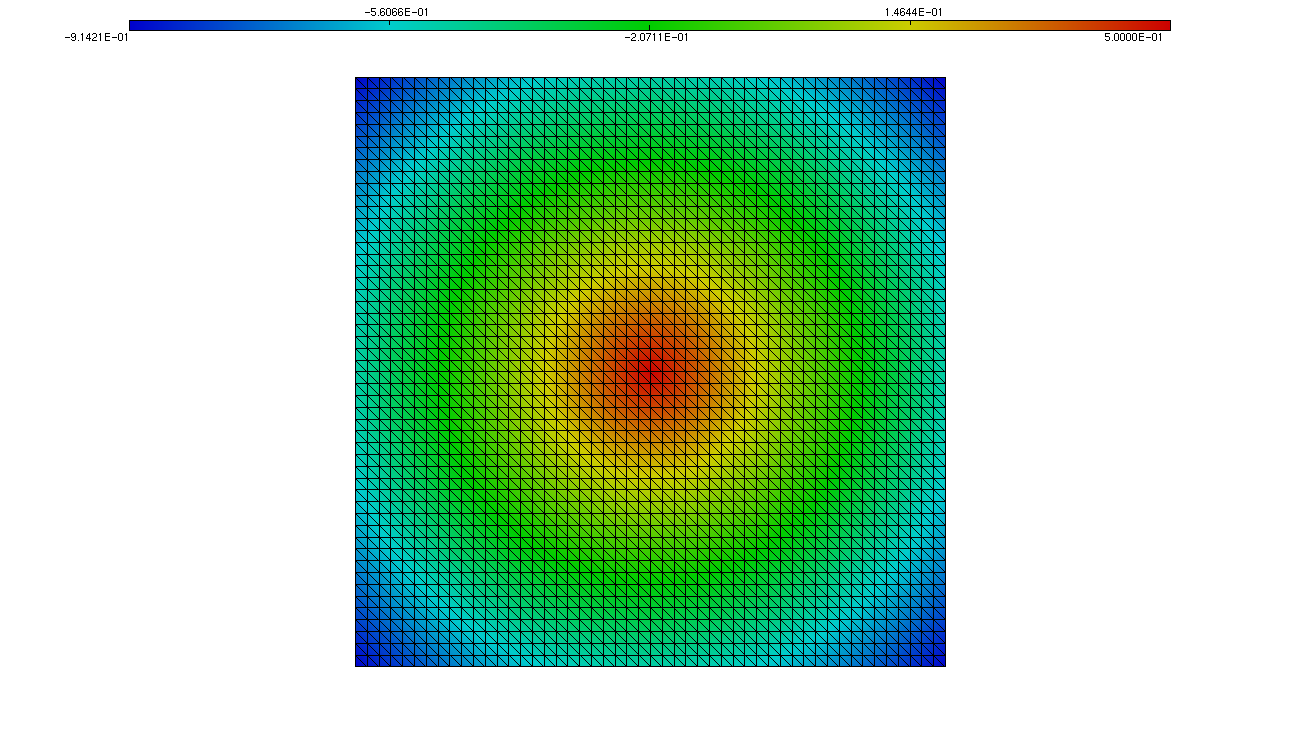
\includegraphics[clip=true, trim = 10cm 0 10cm 0, scale=.25]{Bordeaux/figures/LSinit.png}
		\captionof{subfigure}{Fonction Level Set représentée sur le maillage initial}
	\end{minipage}
	\hfill
	\begin{minipage}[t]{.5\linewidth}
		\centering
		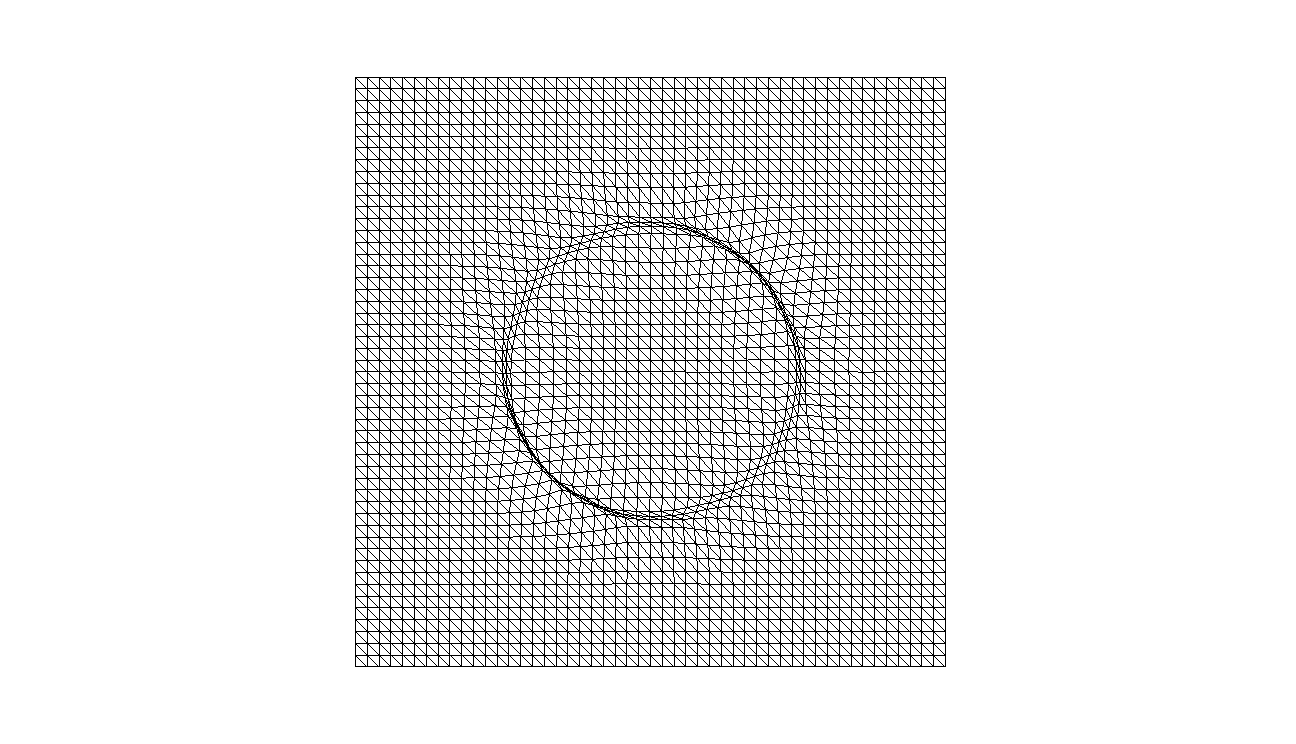
\includegraphics[clip=true, trim = 10cm 0 10cm 0, scale=.25]{Bordeaux/figures/LSadapt.png}
		\captionof{subfigure}{Maillage adapté à la fonction Level Set}
	\end{minipage}
	\captionof{figure}{Exemple d'adaptation à la fonction Level Set \label{fig:exLS}}
\endgroup

\subsection{Construction de la fonction à adapter (avec \(\omega\) donné par l'expression \eqref{eq:omega2})}

\indent Le calcul de \(\omega\) à partir de l'expression \eqref{eq:omega2} est fait en utilisant le gradient et le hessien de la fonction à adapter. Pourtant, dans le cas de la fonction Level Set, l'adaptation ne sera pas faite en considérant \(u=LS\), parce qu'on n'aurait pas de forts gradients, en tenant compte de la lisseté de cette fonction. Ainsi, \(\omega\) ne serait pas capable d'exprimer le raffinement désiré dans chaque partie du maillage. De cette façon, à partir de la fonction Level Set, on va construire une nouvelle fonction qui ait un très fort gradient sur les bords de l'objet.

\indent Idéalement, on construirait une fonction avec un saut, valant \(1\) à l'extérieur et \(-1\) à l'extérieur de l'objet, ce que fournit des très bons raffinements sur la ligne de niveau 0 de la fonction Level Set. Néanmoins, dans la résolution numérique de problèmes de la mécanique des fluides, il est intéressant d'avoir aussi un bon raffinement du maillage sur une couche autour de la surface (la couche limite de l'écoulement), où l'interaction fluide-objet n'est pas négligeable. En effet, pour avoir un calcul précis, un maillage approprié sur la couche limite est requis par la plupart des schémas numériques et logiciels pour les problèmes de fluides \cite{loseille}. Ainsi, on a cherché une fonction plus lisse.

\indent Dans un premier moment, on a défini une fonction avec une variation linéaire entre les deux étages (figure \ref{fig:atan}). Néanmoins, les tests réalisées ont fourni des résultats de mauvaise qualité : étant le gradient constant à l'intérieur de la pente, les points dans cette région (y compris les points les proches du bord de l'objet) n'avaient pas la tendance de bouger, au contraire des points proches des bordes de la pente, dû à la discontinuité du gradient de \(u\). Par conséquent, l'adaptation produisait une maillage avec deux petites couches raffinées, qui ne représentaient pas la surface de l'objet (figure \ref{fig:LSlin}).

\begingroup
  \centering
  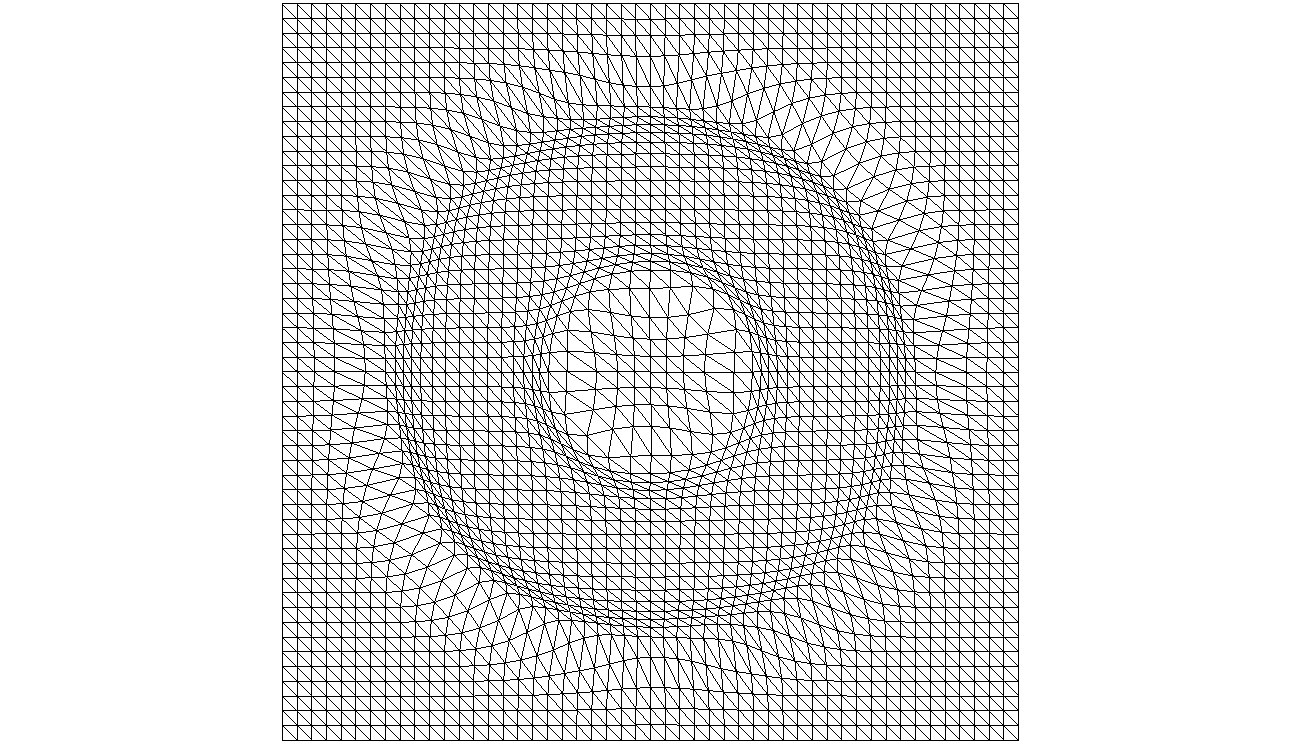
\includegraphics[clip=true, trim = 10cm 0 10cm 0, scale=.25]{Bordeaux/figures/LSlin.png}
  \captionof{figure}{Adaptation à une fonction Level Set modifié avec une variation linéaire \label{fig:LSlin}}
\endgroup

\indent On a ainsi cherché une fonction dont le gradient est plus variable et continue afin de réduire cet effet. On a obtenu des bons résultats en utilisant

\begin{equation}
	\label{eq:atan}
	u(\vecx) = \frac{1}{1.1.107} atan \left(\frac{2LS(\vecx)}{\delta} \right)
\end{equation}

\noindent étant \(2\delta\) la taille de la couche, choisie par l'utilisateur. Cette fonction est représentée dans la figure \ref{fig:atan}.

\begingroup
  \centering
  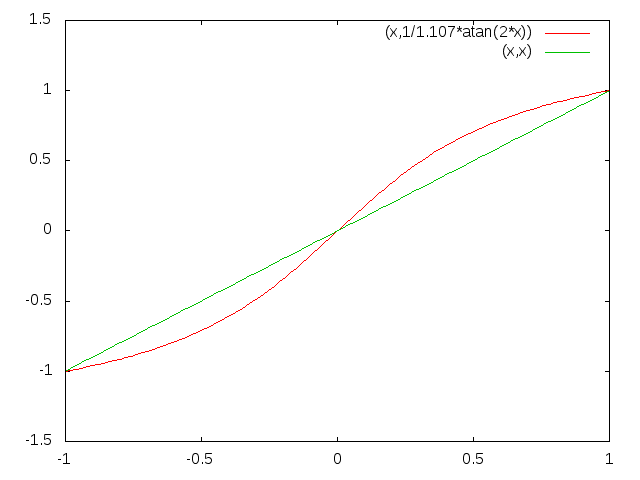
\includegraphics[scale=.4]{Bordeaux/figures/atan.png}
  \captionof{figure}{Comparaison des options pour la lissage de la fonction à adapter   \label{fig:atan}}
\endgroup

\indent On peut jouer aussi avec le paramètre multiplicateur de \(LS(\vecx)/\delta\) à l'intérieur de la fonction tangent. Avec 1, par exemple, on obtient un résultat plus proche de la pente linéaire; avec 5 ou 10, la fonction devient plus discontinue et la couche de raffinement est plus petite. On restera ainsi avec l'option donnée par \eqref{eq:atan}.



\subsubsection{Choix des paramètres}

\indent Afin de chercher les paramètres qui génèrent le meilleur maillage, plusieurs tests on été réalisés : 

\begin{itemize}
	\item Cas test (objet cible): 
	\begin{itemize}
		\item Cercle;
		\item Triangle;
		\item Profil d'une aile (NACA)
	\end{itemize}
	\item Type de maillage
	\begin{itemize}
		\item Structuré;
		\item Non structuré
	\end{itemize}
\end{itemize}

\indent Les meilleurs maillages obtenus on été utilisés pour résoudre un problème d'écoulement autour de l'objet, afin de vérifier l'influence sur les résultats. Les conclusions des tests sont les suivants : 

\begin{itemize}
  \item Pour le calcul de \(\omega\), il faut plutôt utiliser le gradient de \(u\). Le hessien peut être aussi utilisé, mais il a la tendance de créer deux couches raffinées dans les bords de la région de variation de la fonction \(u\) (figure \ref{fig:alphabeta});
  \item Le raffinement d'une certaine région du maillage cause un étirement dans la direction normale à surface des éléments voisins à cette région. Ce résultat n'est pas désirable car on veut plutôt une anisotropie dans la direction de l'écoulement du fluide (figure \ref{fig:anisoNormal}) : l'erreur d'interpolation est plus petit si on a des triangles anisotropes dont le côté le plus long est dans la direction des petites dérivées de deuxième ordre de la solution \cite{rippa}. Ainsi, il est important de avoir une valeur de \(\delta\) assez grande.
  \item Néanmoins, \(\delta\) ne peut être trop grand, car la fonction arctangente s'approche de la pente linéaire, et on n'obtient pas un bon raffinement à l'intérieur de la couche.
\end{itemize}


\begingroup
	\begin{minipage}[t]{.5\linewidth}
		\centering
		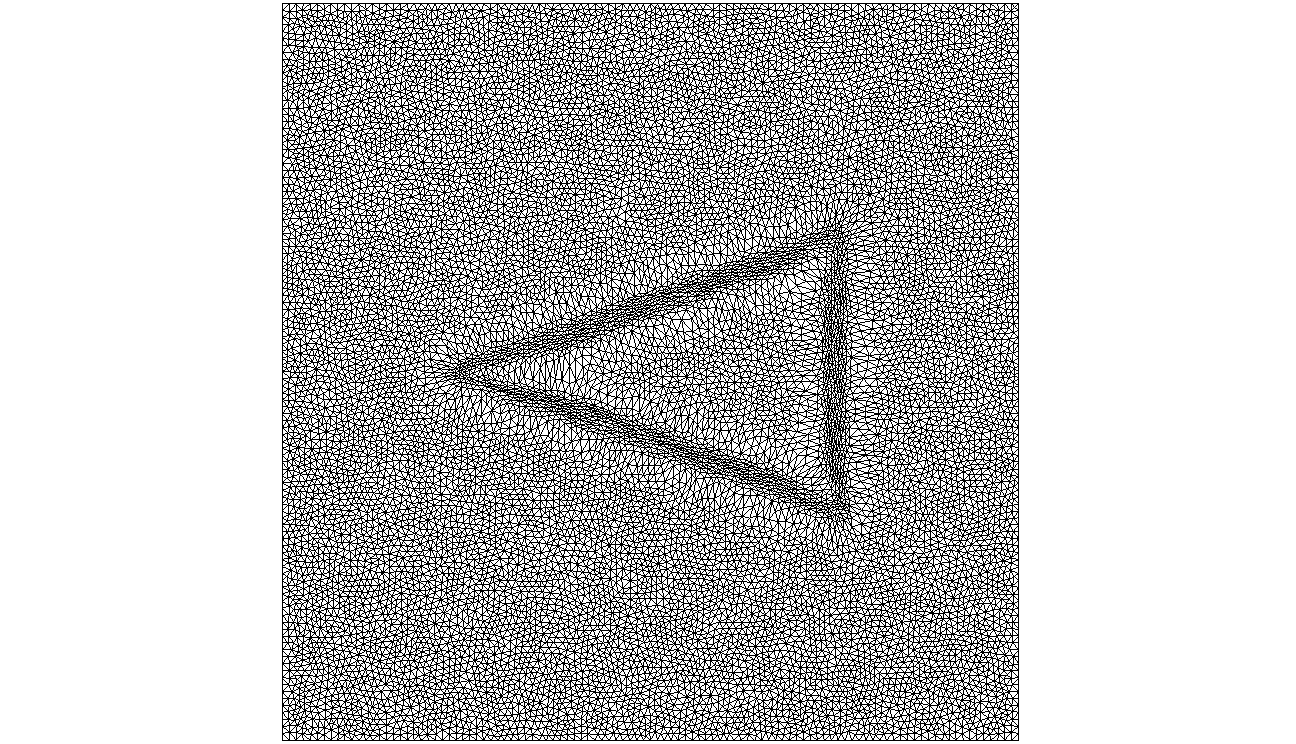
\includegraphics[clip=true, trim = 10cm 0 10cm 0, scale=.25]{Bordeaux/figures/alphabeta0.png}
		\captionof{subfigure}{\(\alpha = 1000, \beta = 0\)}
	\end{minipage}
	\hfill
	\begin{minipage}[t]{.5\linewidth}
		\centering
		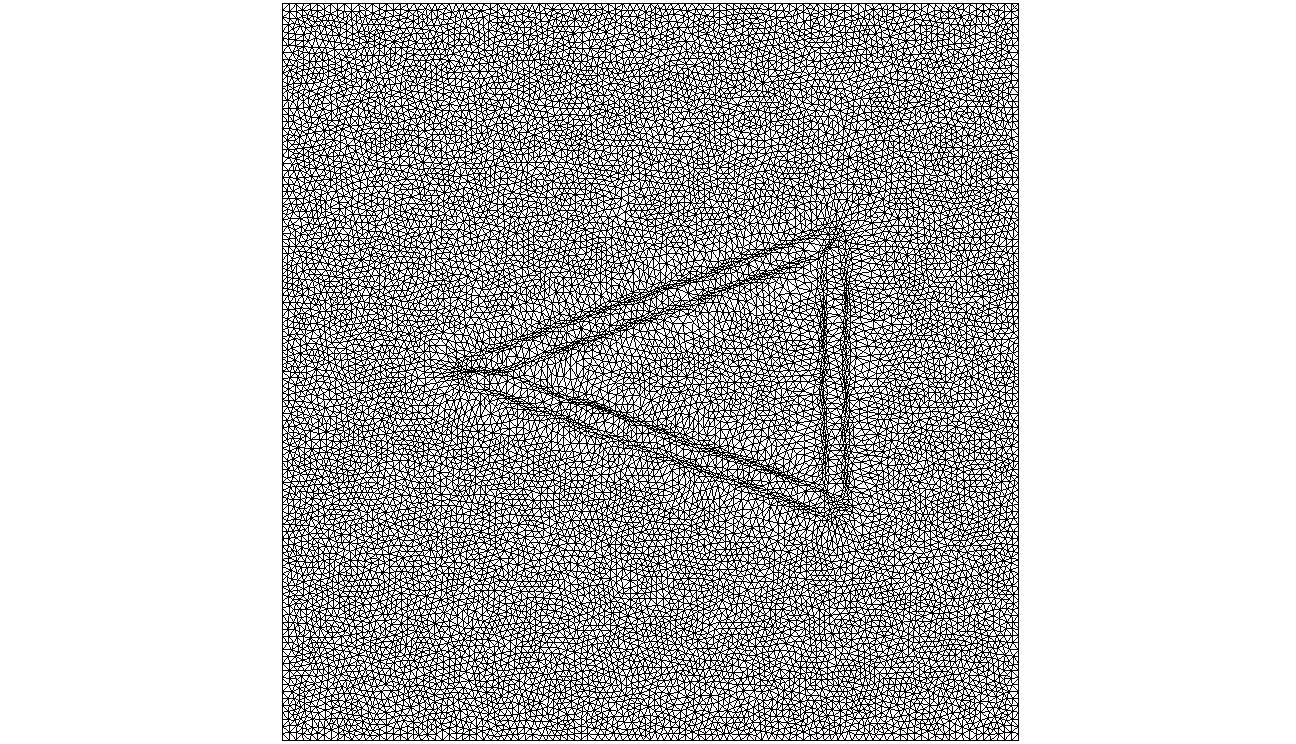
\includegraphics[clip=true, trim = 10cm 0 10cm 0, scale=.25]{Bordeaux/figures/alphabeta1.png}
		\captionof{subfigure}{\(\alpha = 0, \beta = 1000\)}
	\end{minipage}
	\captionof{figure}{Influence des paramètres \(\alpha\) et \(\beta\) sur l'adaptation du maillage (les deux cas ave \(\delta = 0.02\)) \label{fig:alphabeta}}
\endgroup

\begingroup
	\centering
	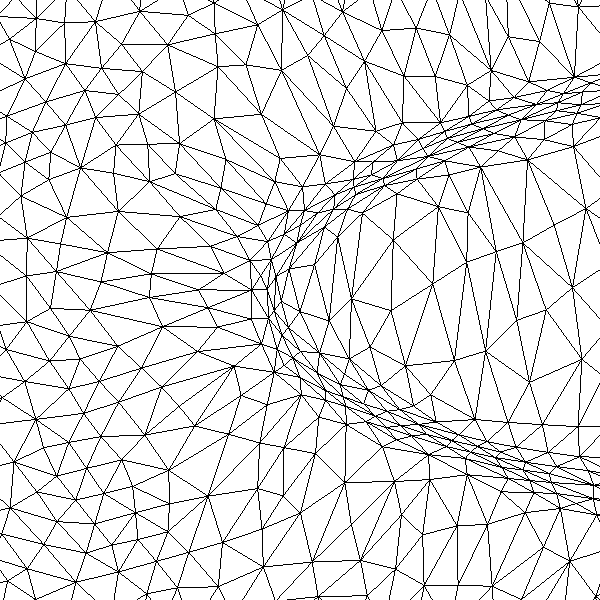
\includegraphics[scale=.25]{Bordeaux/figures/anisoNormal.png}
	\captionof{figure}{Détail d'un maillage obtenu avec \(\delta = 0.005\) \label{fig:anisoNormal}}
\endgroup

\indent En tenant compte de ces conclusions, on recommande l'utilisation des paramètres suivants (on rappelle qu'on utilise toujours les normes du gradient et du hessien normalisés entre 0 et 1) : 

\begin{equation*}
	\boldsymbol{\alpha} = 1000, \qquad 
	\boldsymbol{\beta} = 0, \qquad
	\boldsymbol{\delta} = 0.01,\  0.02
\end{equation*}

\indent On peut aussi faire des adaptations successives, en faisant varier les paramètres, afin d'obtenir d'autres résultats. Par exemple, on peut faire une première adaptation avec \(\delta = 0.02\) pour obtenir une bonne couche raffinée, et après une deuxième avec \(\delta = 0.01\) pour obtenir un raffinement plus précis autour de la surface. 

\indent La figure \ref{fig:example} présente quelques exemples d'adaptation à une fonction Level Set, avec les paramètres présentés ci-dessus, sur un maillage non structuré avec environ 28000 noeuds : 

\begingroup
	\begin{minipage}[t]{.5\linewidth}
    		\centering
		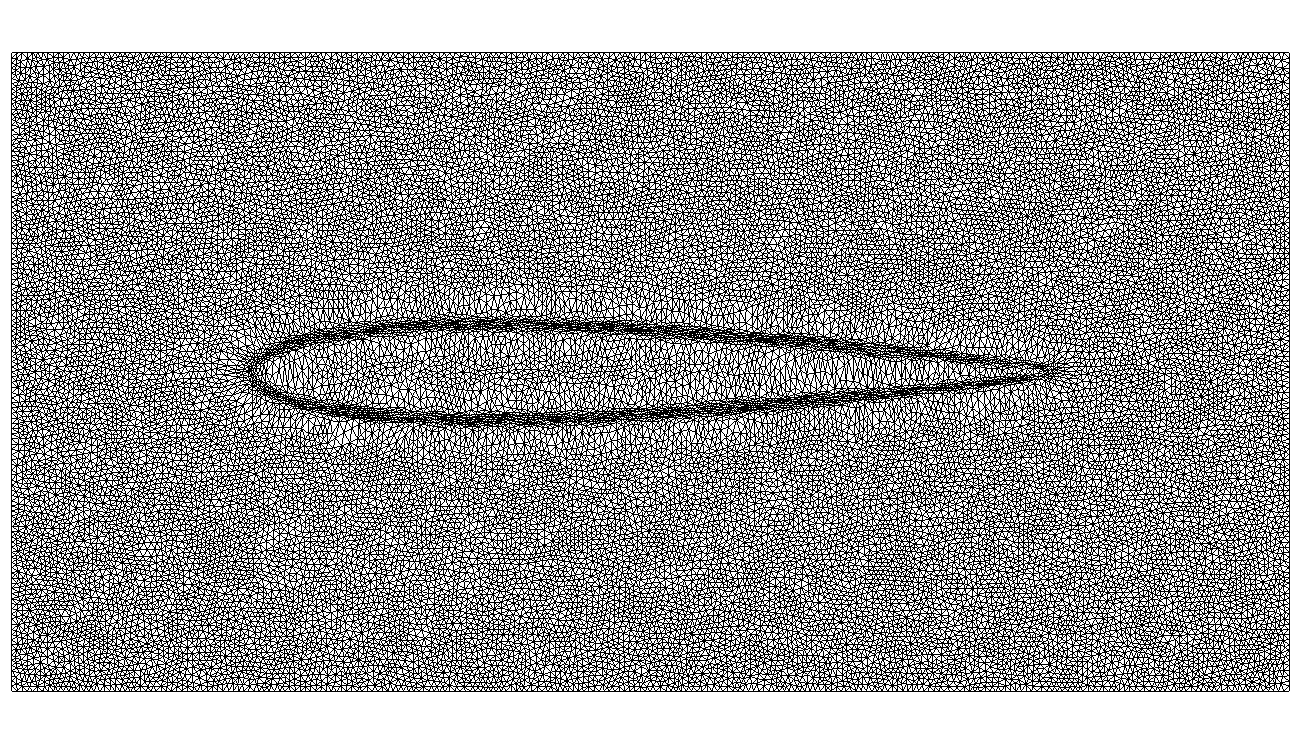
\includegraphics[scale=.15]{{Bordeaux/figures/example1}.png}
		\captionof{subfigure}{\(\delta = 0.01\)}
  	\end{minipage}
	\begin{minipage}[t]{.5\linewidth}
    		\centering
		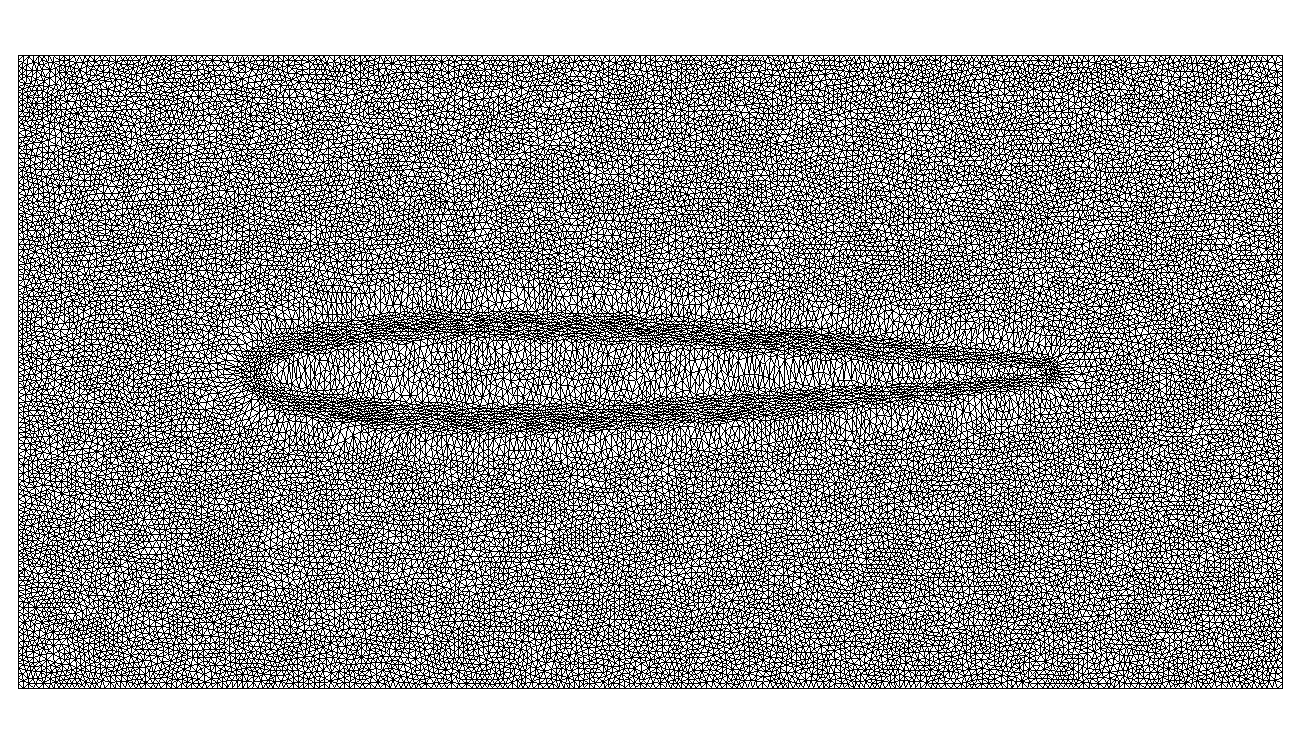
\includegraphics[scale=.15]{{Bordeaux/figures/example2}.png}
		\captionof{subfigure}{\(\delta = 0.02\)}
  	\end{minipage}
  	\captionof{figure}{Exemples d'adaptation à une fonction Level Set \label{fig:example}}
\endgroup


\subsection{Calcul des tailles désirées}

\indent Le calcul des tailles désirées est basée sur la définition d'une métrique pour chaque point du maillage. Il s'agit d'une matrice \(2 \times 2\) (dans le cas bidimensionnel) définie positive symétrique, construite de façon a contrôler l'erreur de la représentation de la solution sur le maillage modifiée \cite{leo}.


\indent La description détaillé de la définition, calcul et interprétation géométrique de la métrique seront faites dans la section \ref{sec:adapPhysique}, pour l'adaptation à une solution physique. Dans le cas de l'adaptation Level Set, on a implémenté un calcul simple des tailles désirées, en se basant sur la méthode utilisée par \cite{ducrot}, qui permet de contrôler la distance de Hausdorff entre la surface de l'objet et sa représentation. En faisant attention toujours à l'importance, pour une bonne adaptation,  de créer une fonction \(\omega\) qui soit au même temps assez lisse et qui présente des variations qui permettent le mouvement des noeuds, on définit, avec le paramètre \(\delta\), des couches pour l'imposition des tailles : 

\begin{equation*}
	\hdes (\vecx_i) =
	\begin{cases}
		\hm \ \ \ si \ \ |LS(\vecx_i)| \leq \frac{\delta}{2} \\
		2\hm \ \ \ si \ \ \frac{\delta}{2} \leq |LS(\vecx_i)|  \leq \delta \\
		\hM \ \ \ sinon
	\end{cases}
\end{equation*}

\noindent et on lisse les tailles sur le maillage avec le logiciel \emph{MMG}, en imposant une gradation de 10\%.

\subsubsection{Résultats}

\indent La figure \ref{fig:adaptMet} illustre l'adaptation Level Set basée sur l'imposition de tailles désirées à chaque noeud.

\begingroup
	\begin{minipage}[t]{.5\linewidth}
		\centering
		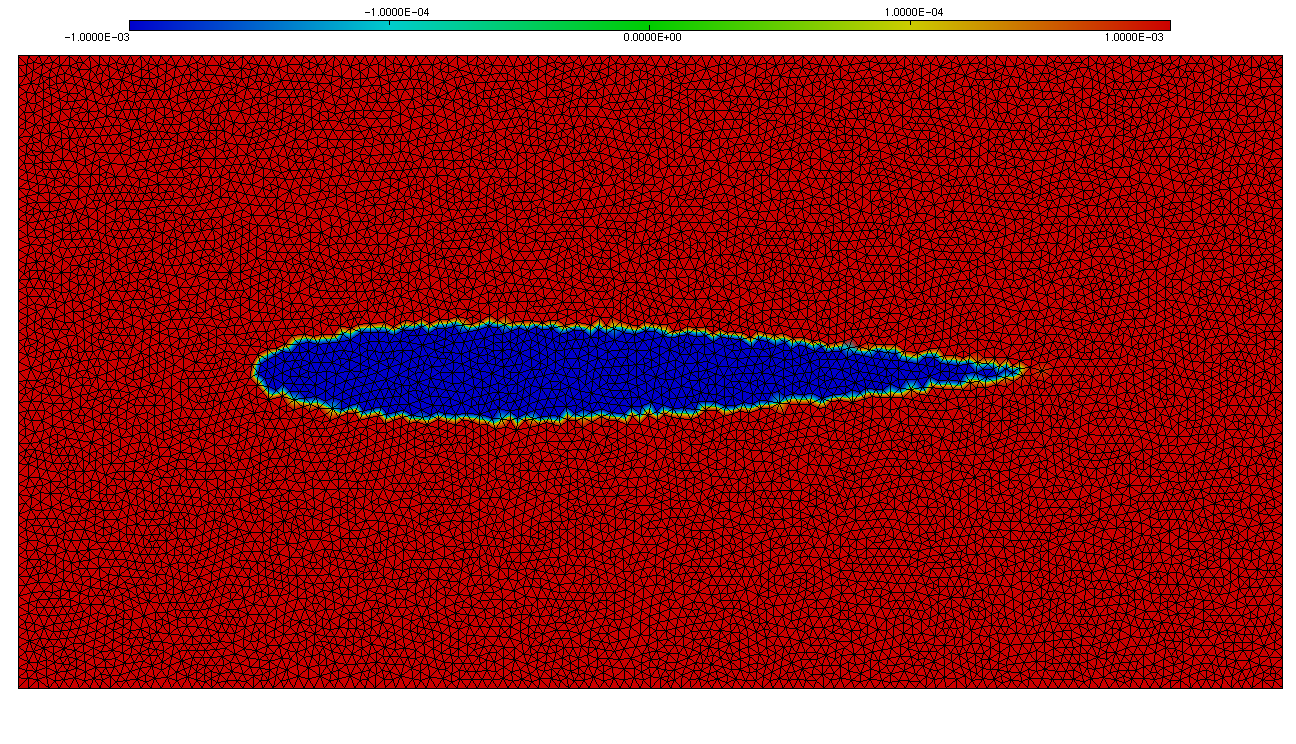
\includegraphics[scale=.15]{Bordeaux/figures/metLSNacaLS.png}
		\captionof{subfigure}{Fonction Level Set}
	\end{minipage}
	\hfill
	\begin{minipage}[t]{.5\linewidth}
		\centering
		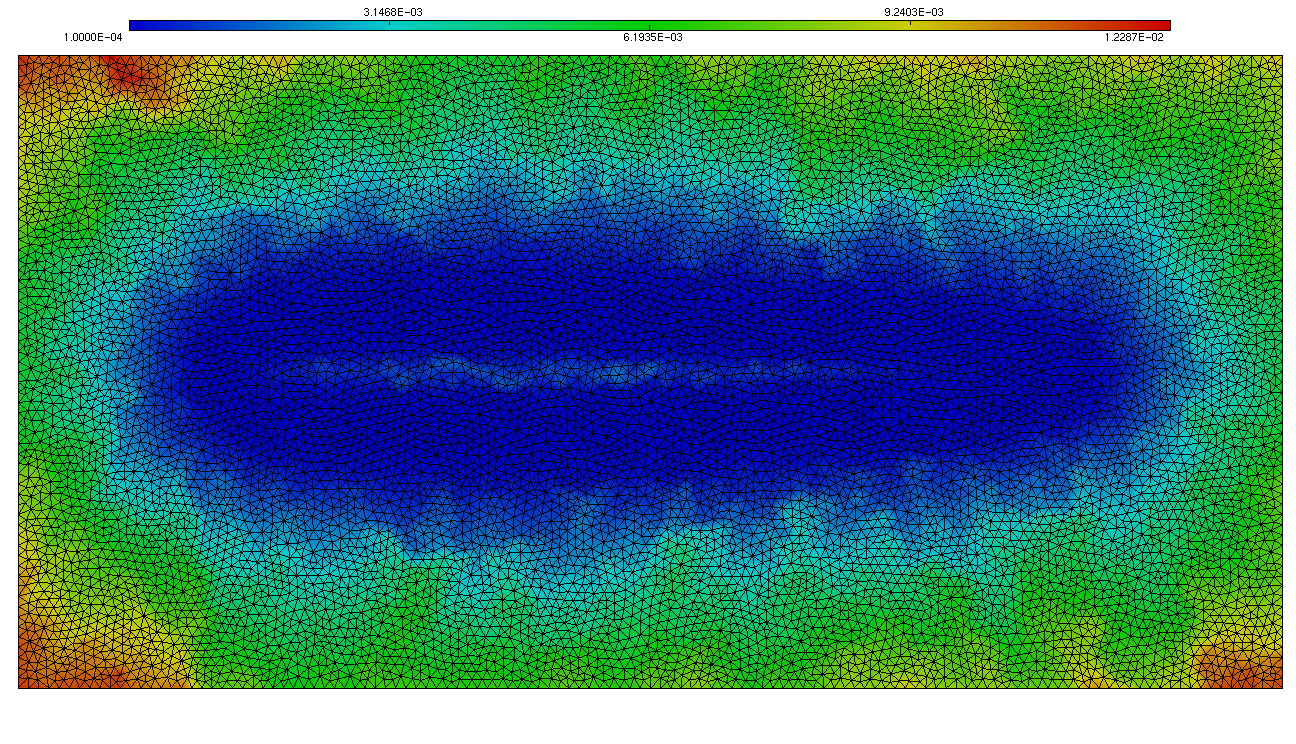
\includegraphics[scale=.15]{Bordeaux/figures/metLSNacaMet.png}
		\captionof{subfigure}{Tailles désirées}
	\end{minipage}	
	\begin{minipage}[t]{1.\linewidth}
		\centering
		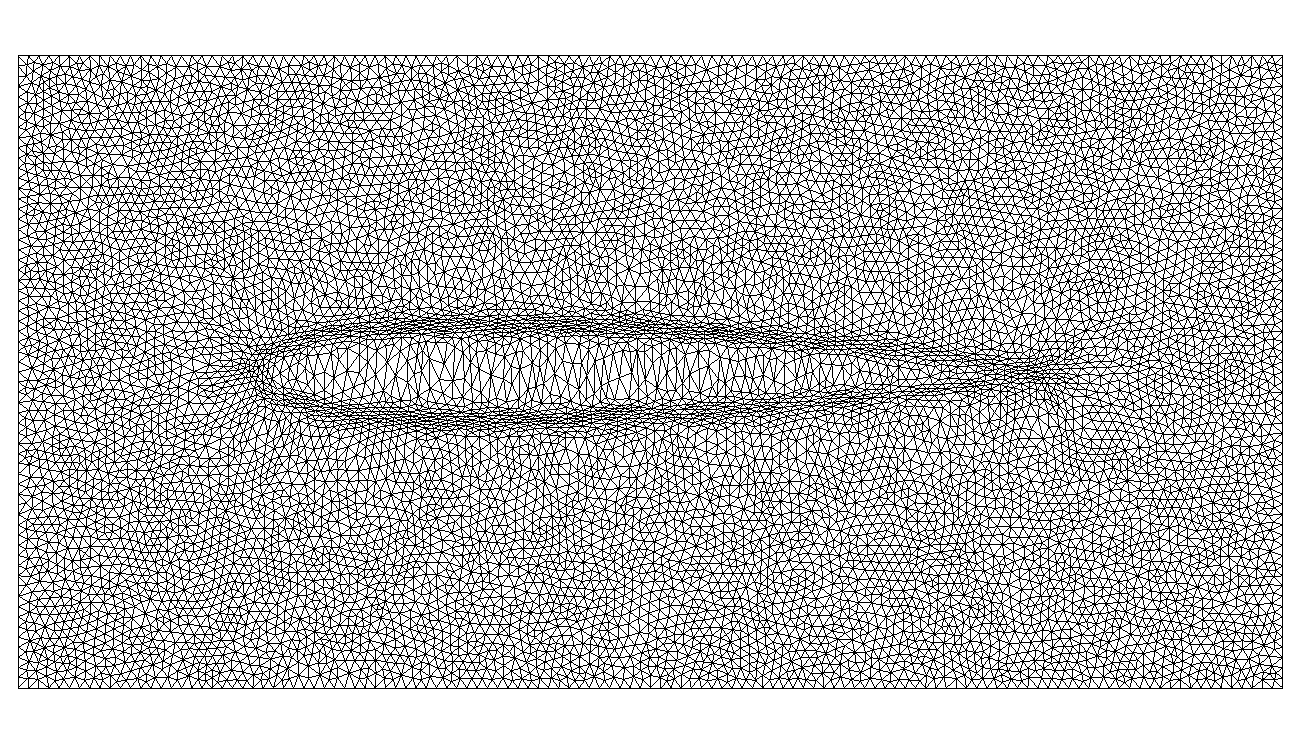
\includegraphics[scale=.2]{Bordeaux/figures/metLSNacaAdapt.png}
		\captionof{subfigure}{Maillage adapté (20 itérations)}
	\end{minipage}	
	\captionof{figure}{Adaptation à une fonction Level Set à partir de l'imposition des tailles désirées \label{fig:adaptMet}}
\endgroup


\subsection{Relaxation et qualité du maillage}

\indent Pendant la résolution du système linéaire, on fait, si nécessaire, une relaxation des déplacements calculés afin d'éviter le croisement des noeuds et la conséquente occurrence d'aires négatives. Néanmoins, en dépendant du maillage de départ (par exemple, un maillage déjà raffiné), la relaxation est trop contraignant et impose l'arrêt de l'algorithme lors des premières itérations. Parfois cela est provoqué par un petit nombre d'éléments.

\indent On a ainsi implémenté, dans les premières itérations, un prétraitement d'optimisation, selon le schéma suivant :

\begin{itemize}
  \item Si le numéro de l'itération actuelle n'est pas supérieur à \(iter_{optim}\) : 
  \begin{enumerate}
    \item Identifier tous les éléments qui demanderont de la relaxation;
    \item Classifier ces éléments selon un critère de qualité (mesure de l'anisotropie);
    \item Optimiser les \(n_{optim}\) éléments les plus critiques de cette liste
  \end{enumerate}   
\end{itemize}

\indent L'optimisation réalisée consiste en, itérativement, approcher chaque noeud \(i\) de l'élément concerné du barycentre des noeuds voisins de \(i\). L'optimisation est arrêtée dès qu'aucun des trois noeuds de l'élément bouge au dessus d'un seuil, ou qu'au moins un des noeuds n'arrive pas à réduire l'anisotropie au dessous d'une certaine pourcentage, par rapport au début de l'itération.

\indent La figure \ref{fig:optim} montre le résultat de son application sur un élément : 

\begingroup
	\begin{minipage}[t]{.5\linewidth}
    		\centering
		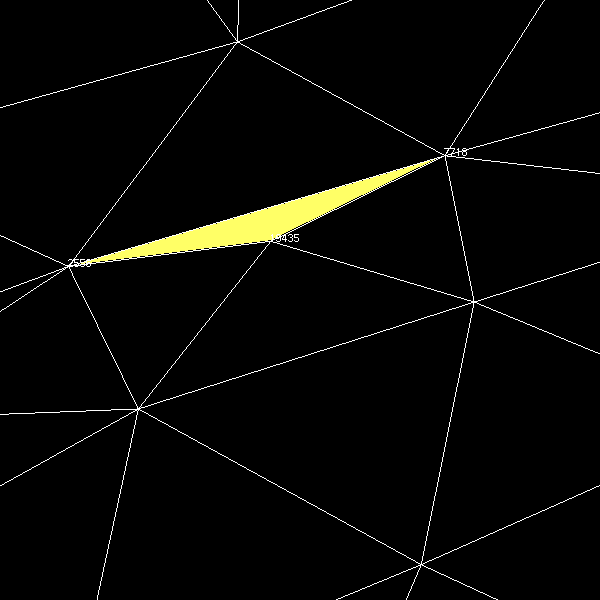
\includegraphics[scale=.25]{{Bordeaux/figures/optim_avant}.png}
		\captionof{subfigure}{Avant l'optimisation}
  	\end{minipage}
  	\hfill
	\begin{minipage}[t]{.5\linewidth}
    		\centering
		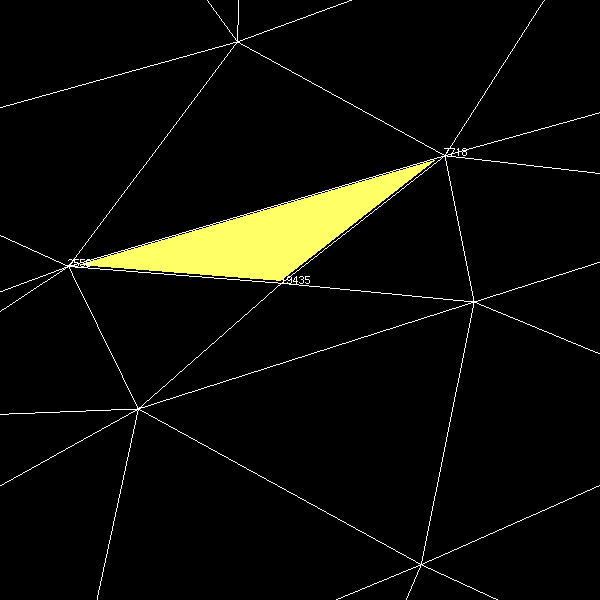
\includegraphics[scale=.25]{{Bordeaux/figures/optim_apres}.png}
		\captionof{subfigure}{Après l'optimisation}
  	\end{minipage}
  	\captionof{figure}{Résultat de l'optimisation d'un élément \label{fig:optim}}
\endgroup

\indent Pour que le prétraitement ne soit pas très coûteux, on a choisi \(n_{optim} = 10\) e \(iter_{optim} = 2\). Les tests réalisés montrent des très bons résultats quand l'algorithme s'arrête au début de l'exécution, et avec l'optimisation on arrive à tourner tous les itérations. Néanmoins, si appliqué sur un maillage de bonne qualité et qui ne demande pas une forte relaxation, les gains sont en général petits (ou même on perd un peu de la qualité du résultat final).


\subsection{Adaptation 3D}

\indent Après le développement et validation du modèle bidimensionnel décrit jusqu'ici, avec l'obtention de bons résultats d'adaptation des maillages, on l'a étendu au cas tridimensionnel. Du point de vue théorique, cette extension est assez simple, étant le modèle toujours décrit par le problème \eqref{eq:systeme}. Le développement de sa formulation faible reste aussi la même, et on se ramène ainsi à la résolution des systèmes linéaires

\begin{equation*}
	\begin{cases}
		Kx = 0 \\
		Ky = 0 \\
		Kz = 0
	\end{cases}
\end{equation*}

\indent Comme ces systèmes sont indépendants et ont la même forme, l'extension du cas 2D au 3D a été également simple du point de vue de l'implémentation. En effet, parmi les calculs décrits en détail dans les sous-sections \ref{subsec:calculK} et \ref{subsec:jacobi}, l'unique modification concerne le calcul des vecteurs normaux (\((\nabref \phii)^T = \frac{\normT{i}}{d!|T|}\), avec \(d=3\)). Ainsi, les éléments de la matrice \(K\) sont donnés par


\begin{equation*}
\begin{gathered}
\begin{aligned}
	k_{ij} & = \iDomh{ \omega \nabref \phii  \cdot \nabref \phij } = \sum_{T \ni i} {\iT{ \omega \nabref \phii \cdot \nabref \phij }} = \\
	       &  = \sum_{T \ni i}
	              { 
	                     { |T|\omega^T \frac{\normT{i}\cdot \normT{j}}{(3!|T|)^2}
	                     }
	              }
	          = \sum_{T \ni i}
	              { 
	                     { \omega^T \frac{\normT{i}\cdot \normT{j}}{36|T|}
	                     }
	              }	              
\end{aligned}
\end{gathered}
\end{equation*}

\indent On présente dans les figures \ref{fig:adaptSphere} à \ref{fig:adaptHole} quelques résultats de l'adaptation Level Set tridimensionnelle, à partir de l'imposition des tailles désirées. Les fonctions Level Set utilisées sont celles de la figure \ref{fig:LS}. Malgré les résultats analogues au cas 2D et cohérents avec les objectifs ici proposés, l'adaptation 3D a des limitations plus fortes concernant le nombre de points du maillage, qui peut devenir très grande pour qu'on ait un maillage suffisamment fine pour la bonne représentation de la fonction Level Set, et la relaxation de l'adaptation, puisque le dégrée de liberté additionnel peut conduire plus rapidement au croisement des noeuds.

\indent Les domaines de départ sont plus raffinées dans les régions où se trouve l'objet, afin de minimiser l'influence des bords sur l'adaptation. Le logiciel \emph{MMG} a été utilisé pour les générer, en imposant une taille minimale \(hmin =  0.05\) et une gradation de \(hgrad = 1.1\) de la variation de las tailles. Les adaptations ont été faites avec \(\delta\) entre 0.05 et 0.07.

\begingroup
	\begin{minipage}{.3\linewidth}
		\centering
		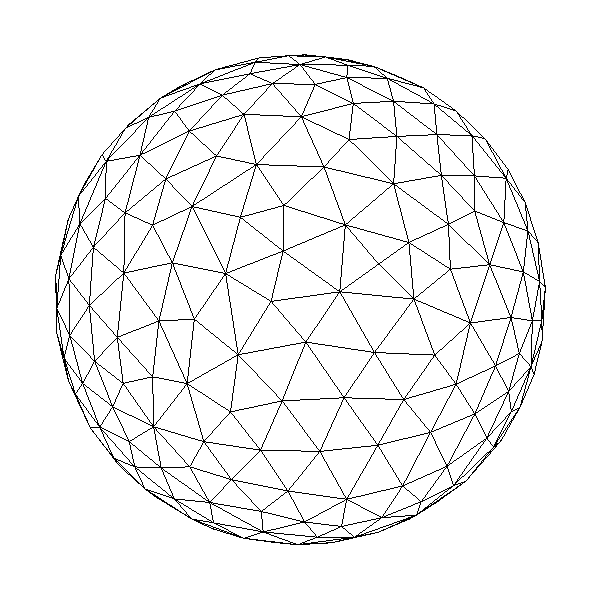
\includegraphics[scale=.2]{Bordeaux/figures/3D/sphereLS.png}
		\captionof{subfigure}{Sphere \label{fig:sphereLS}}
	\end{minipage}
	\hfill
	\begin{minipage}{.3\linewidth}
		\centering
		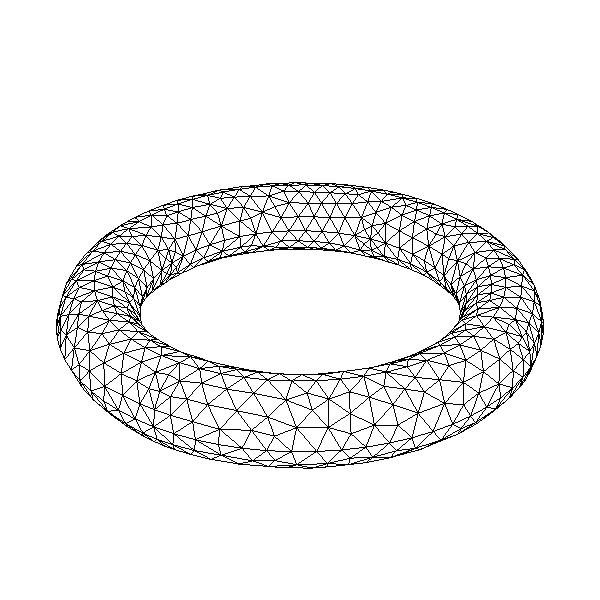
\includegraphics[scale=.2]{Bordeaux/figures/3D/torusLS.png}
		\captionof{subfigure}{Tore \label{fig:torusLS}}
	\end{minipage}
	\hfill
	\begin{minipage}{.3\linewidth}
		\centering
		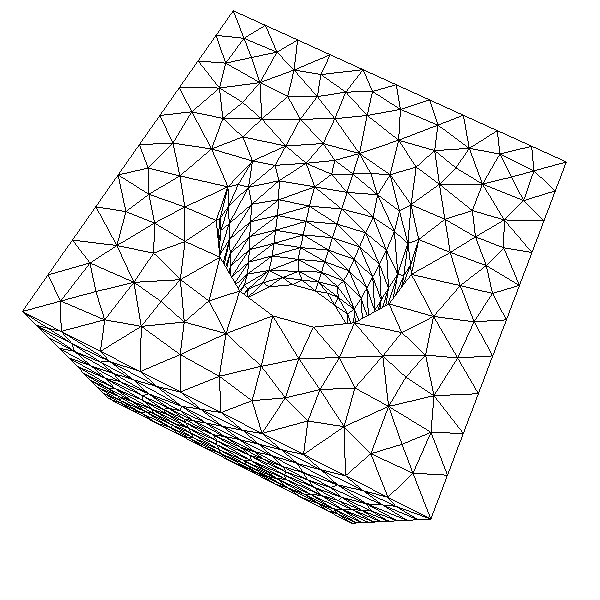
\includegraphics[scale=.2]{Bordeaux/figures/3D/holeLS.png}
		\captionof{subfigure}{Boîte avec un trou \label{fig:holeLS}}
	\end{minipage}
	\captionof{figure}{Fonctions Level Set utilisées \label{fig:LS}}
\endgroup

\begingroup
	\begin{minipage}[t]{.5\linewidth}
		\centering
		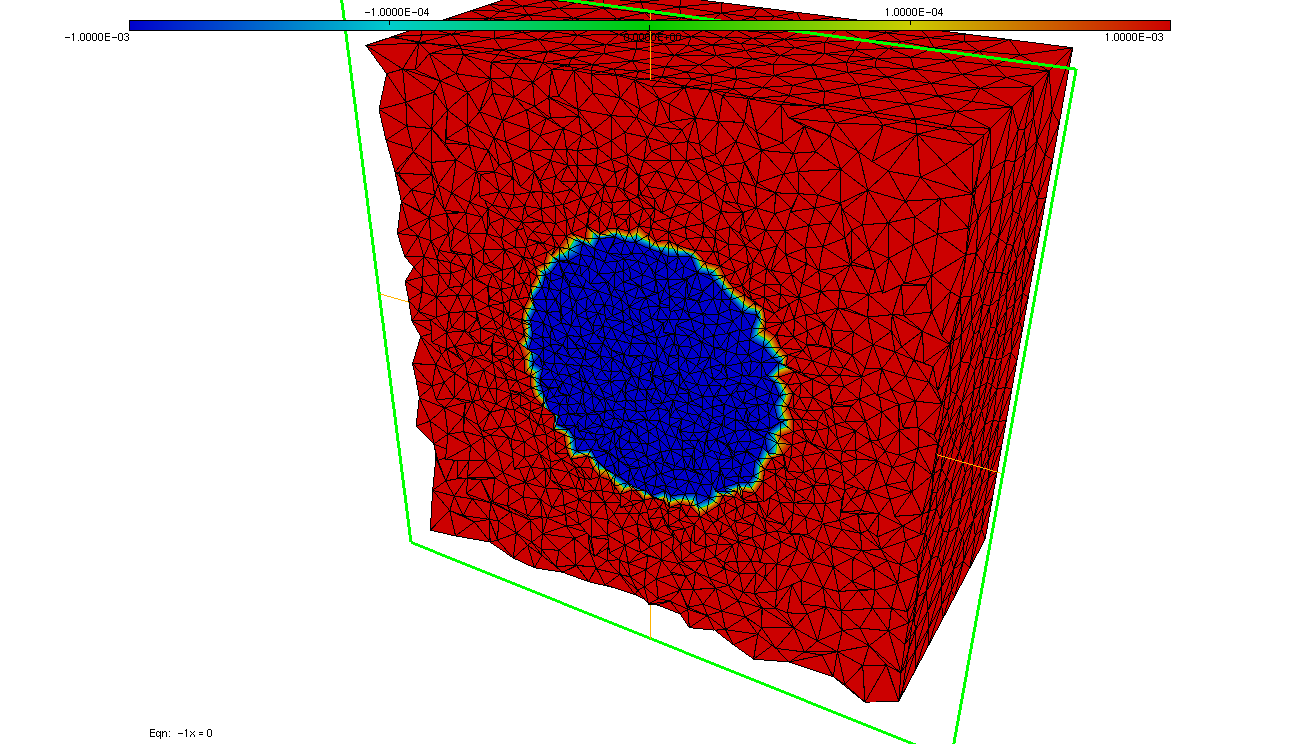
\includegraphics[clip=true, trim=5cm 0 2cm 0, scale=.2]{Bordeaux/figures/3D/sphereDomLS.png}
		\captionof{subfigure}{Fonction Level Set}
	\end{minipage}
	\hfill
	\begin{minipage}[t]{.5\linewidth}
		\centering
		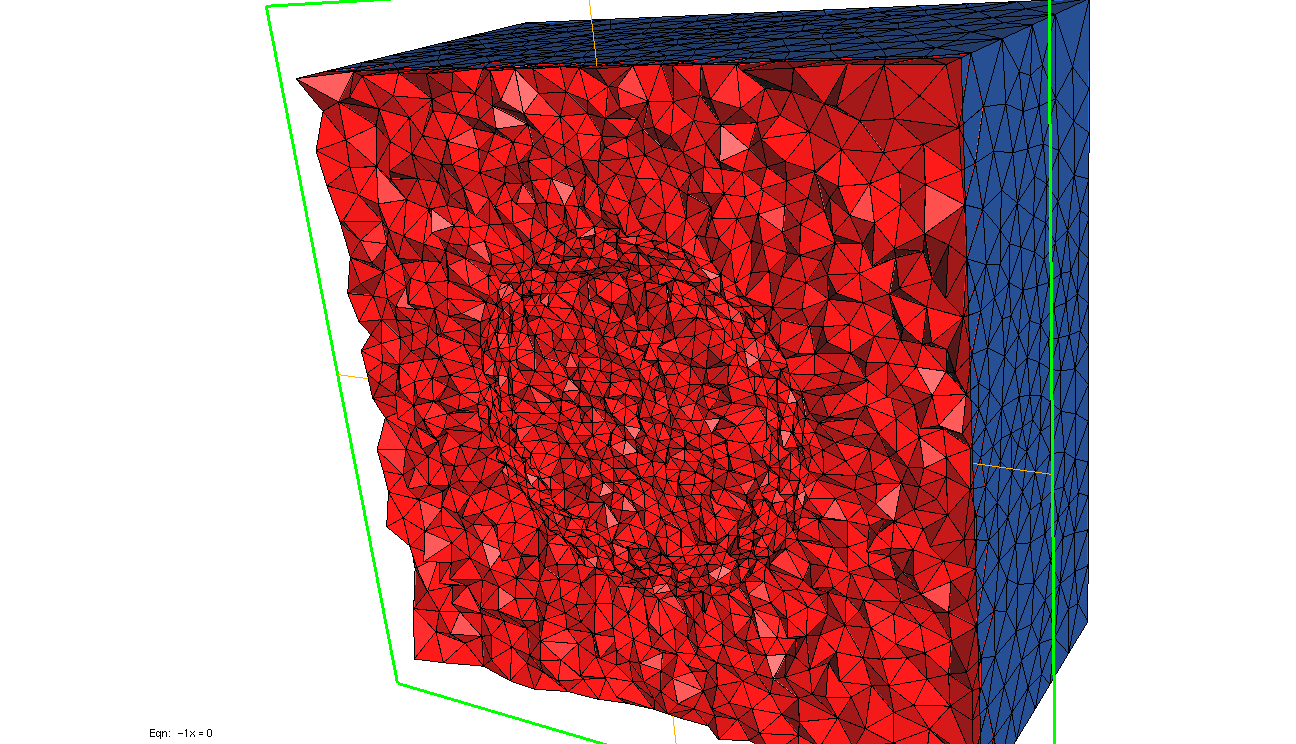
\includegraphics[clip=true, trim=5cm 0 5cm 0, scale=.2]{Bordeaux/figures/3D/sphereAdapt.png}
		\captionof{subfigure}{Maillage adapté (7 itérations)}
	\end{minipage}
	\captionof{figure}{Adaptation du maillage à la sphère (environ 34000 noeuds) \label{fig:adaptSphere}}
\endgroup

\begingroup
	\begin{minipage}[t]{.5\linewidth}
		\centering
		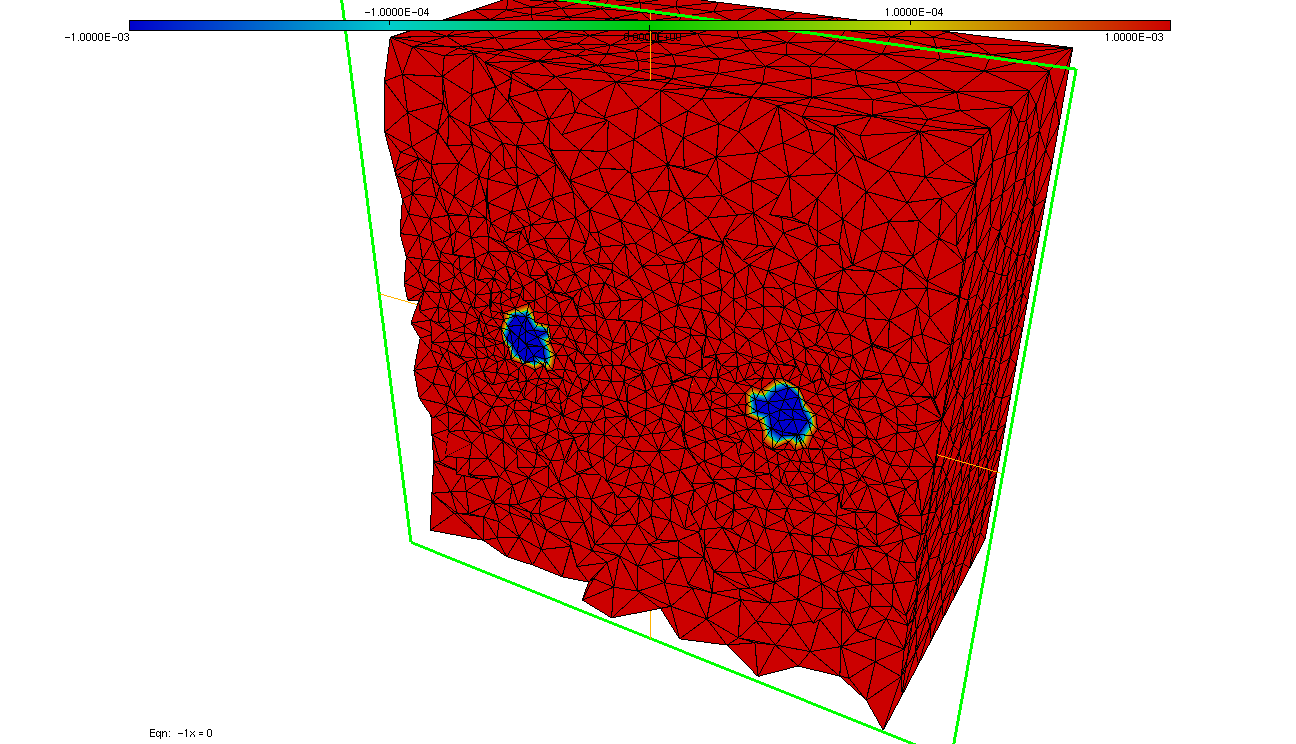
\includegraphics[clip=true, trim=5cm 0 2cm 0, scale=.2]{Bordeaux/figures/3D/torusDomLS1.png}
		\captionof{subfigure}{Fonction Level Set}
	\end{minipage}
	\hfill
	\begin{minipage}[t]{.5\linewidth}
		\centering
		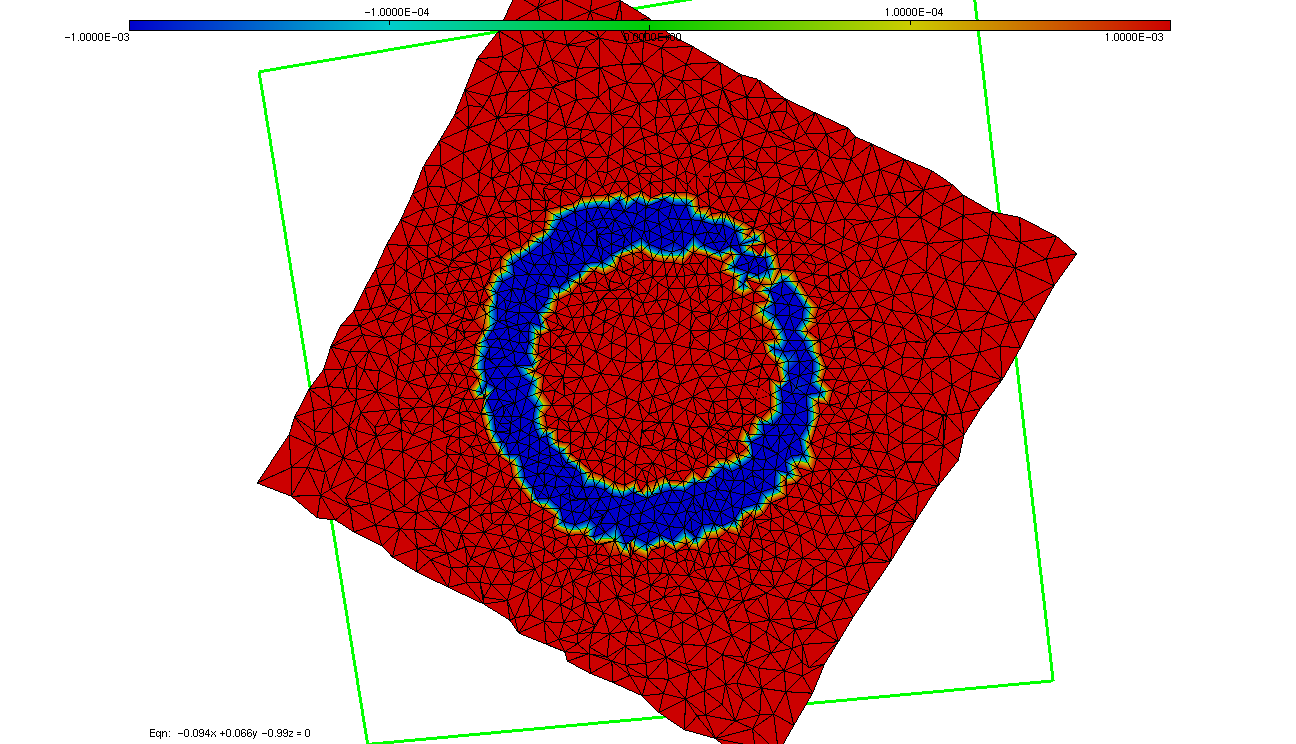
\includegraphics[clip=true, trim=5cm 0 2cm 0, scale=.2]{Bordeaux/figures/3D/torusDomLS2.png}
		\captionof{subfigure}{Fonction Level Set}
	\end{minipage}
	\begin{minipage}[t]{.5\linewidth}
		\centering
		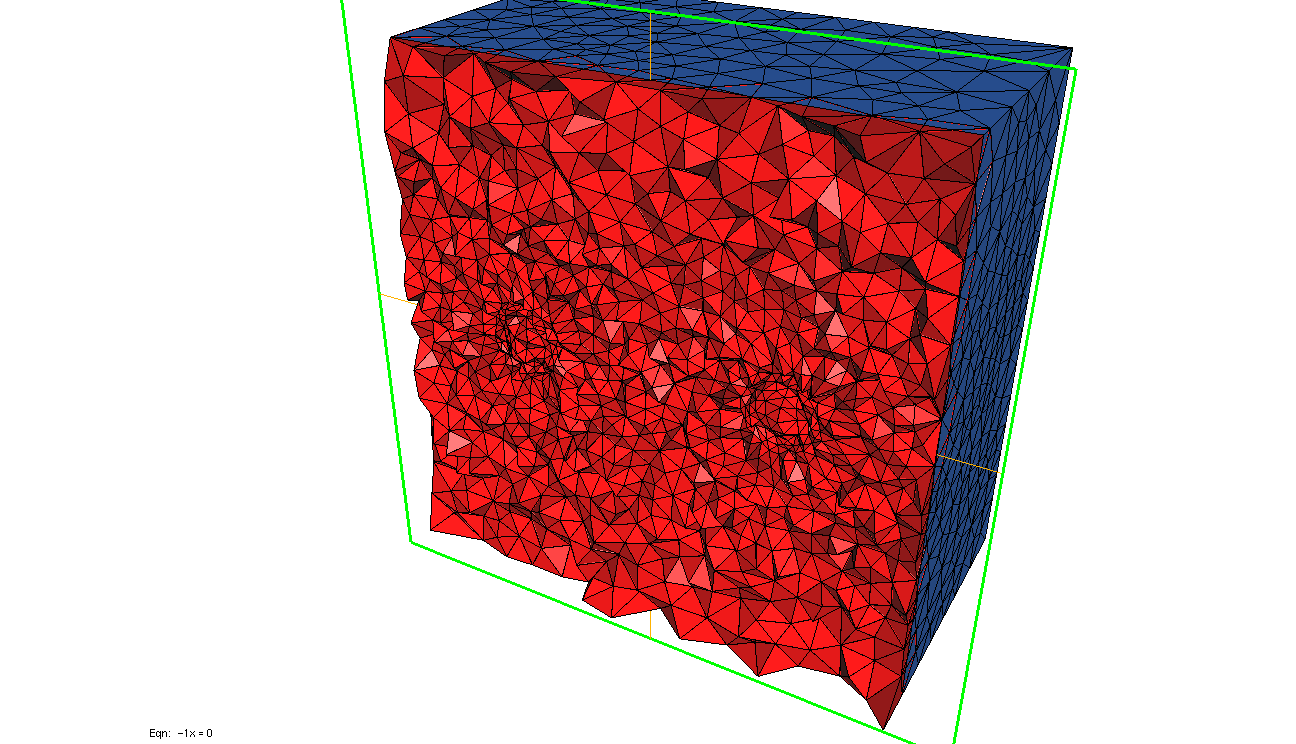
\includegraphics[clip=true, trim=5cm 0 2cm 0, scale=.2]{Bordeaux/figures/3D/torusAdapt2.png}
		\captionof{subfigure}{Maillage adapté (8 itérations)}
	\end{minipage}
	\hfill
	\begin{minipage}[t]{.5\linewidth}
		\centering
		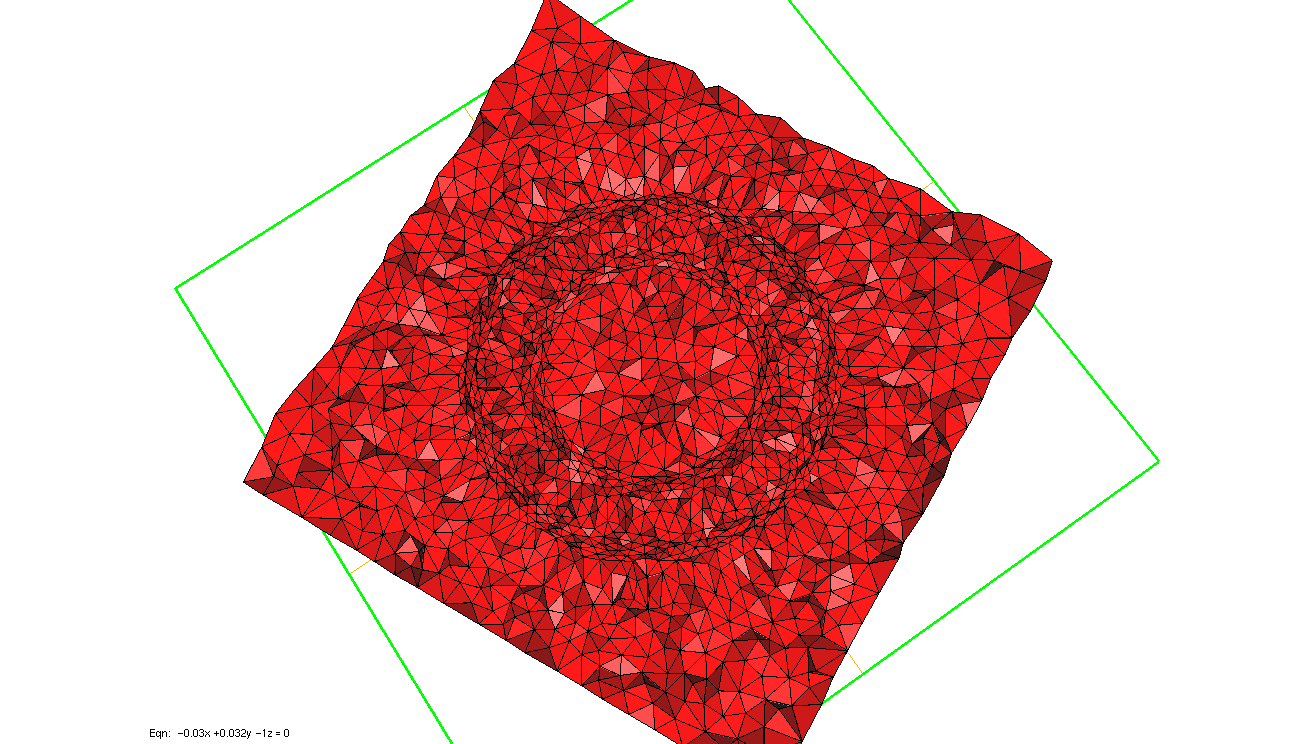
\includegraphics[clip=true, trim=5cm 0 2cm 0, scale=.2]{Bordeaux/figures/3D/torusAdapt1.png}
		\captionof{subfigure}{Maillage adapté (8 itérations)}
	\end{minipage}
	\captionof{figure}{Adaptation du maillage au tore (environ 25000 noeuds) \label{fig:adaptTorus}}
\endgroup

\begingroup
	\begin{minipage}[t]{.5\linewidth}
		\centering
		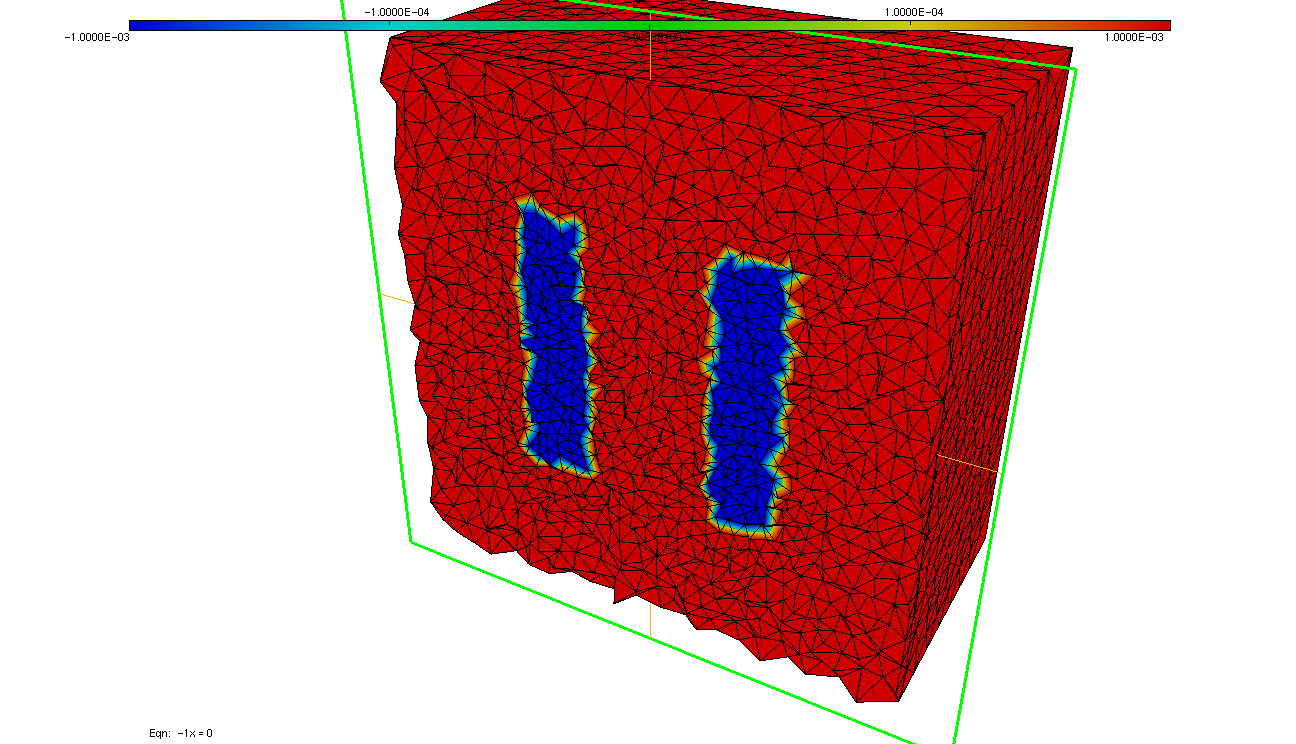
\includegraphics[clip=true, trim=5cm 0 2cm 0, scale=.2]{Bordeaux/figures/3D/holeDomLS1.png}
		\captionof{subfigure}{Fonction Level Set}
	\end{minipage}
	\begin{minipage}[t]{.5\linewidth}
		\centering
		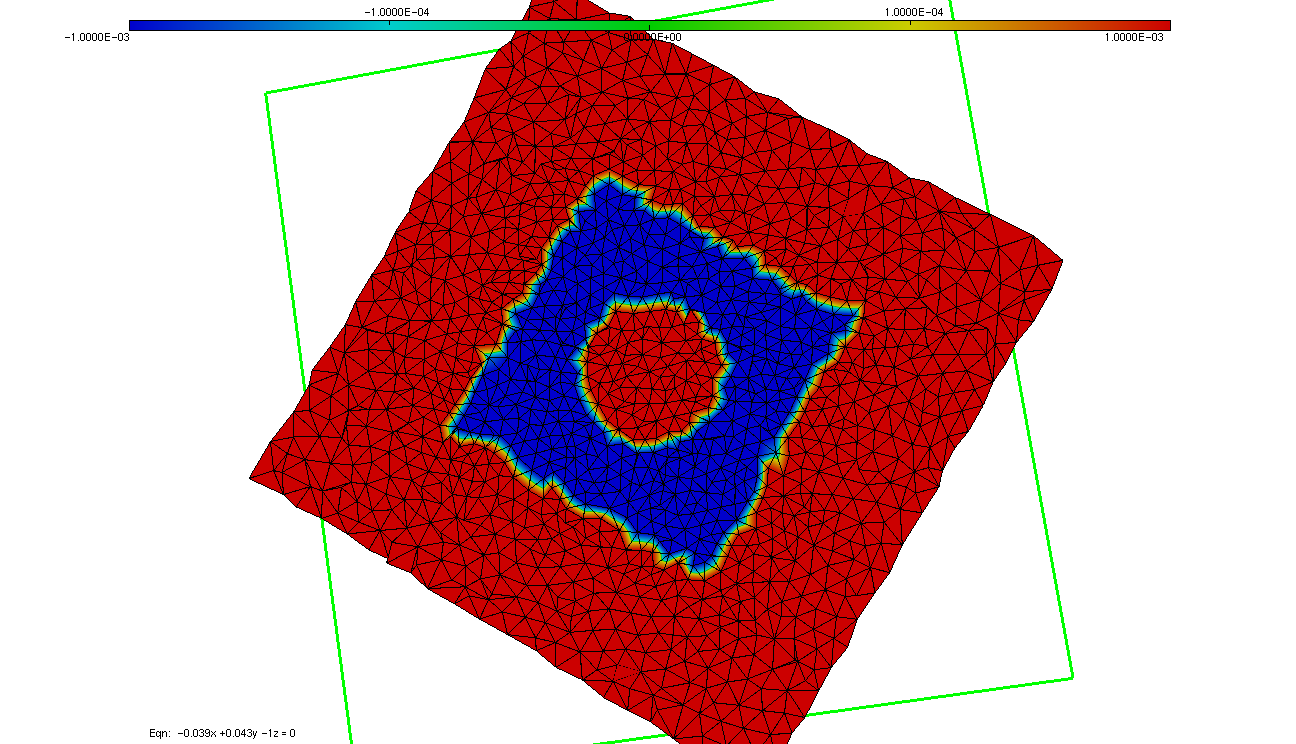
\includegraphics[clip=true, trim=5cm 0 2cm 0, scale=.2]{Bordeaux/figures/3D/holeDomLS2.png}
		\captionof{subfigure}{Fonction Level Set}
	\end{minipage}
	\begin{minipage}[t]{.5\linewidth}
		\centering
		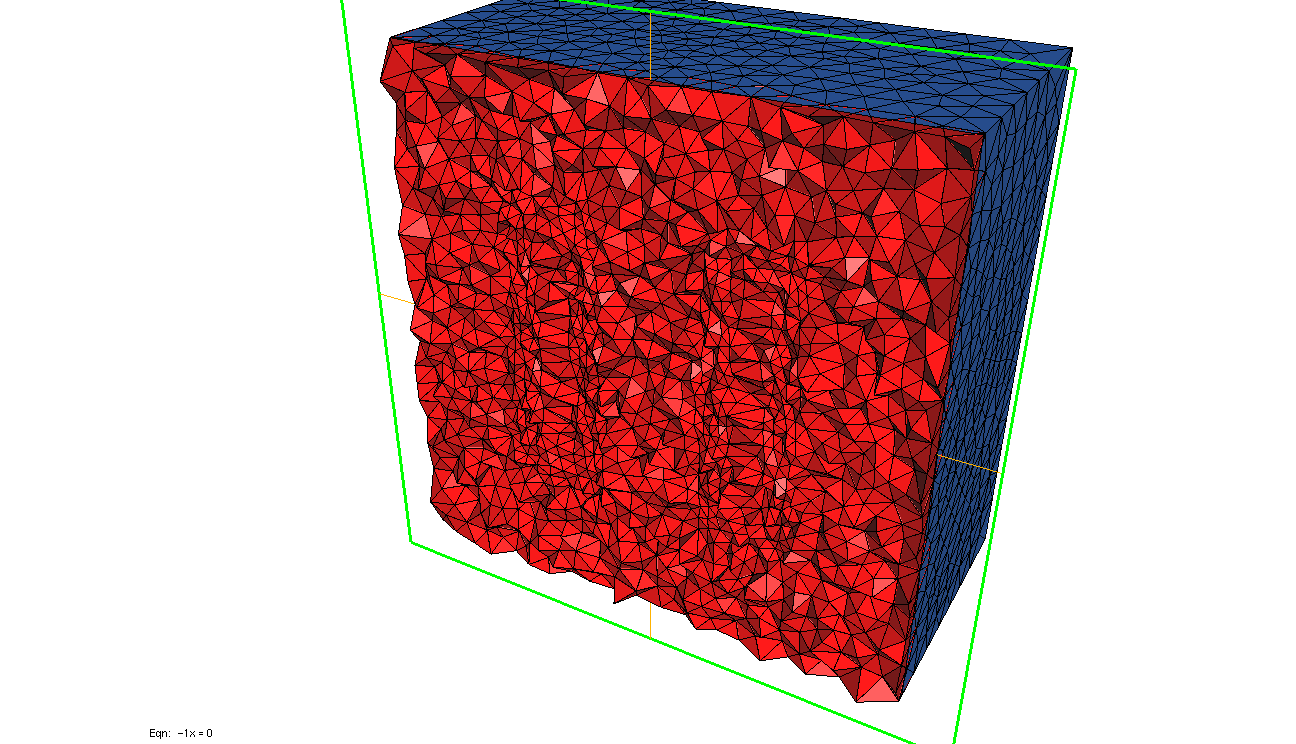
\includegraphics[clip=true, trim=5cm 0 2cm 0, scale=.2]{Bordeaux/figures/3D/holeAdapt1.png}
		\captionof{subfigure}{Maillage adapté (5 itérations)}
	\end{minipage}
	\begin{minipage}[t]{.5\linewidth}
		\centering
		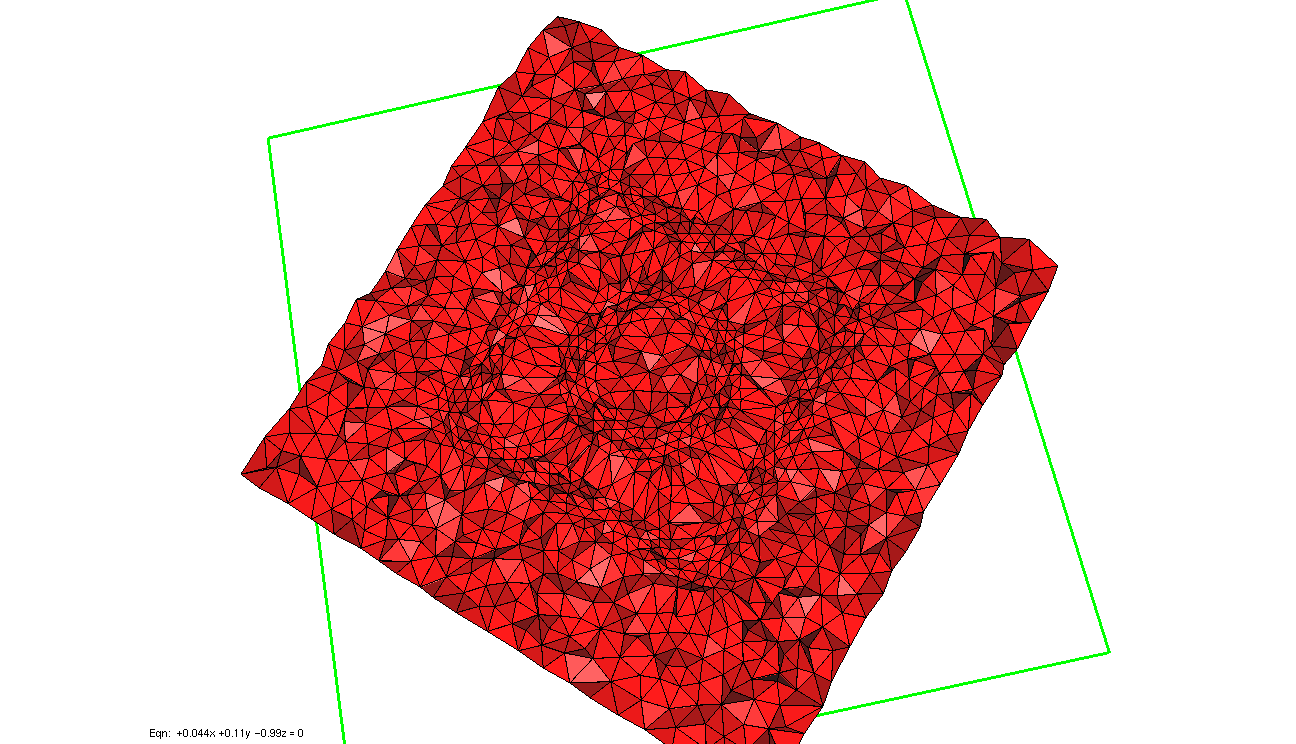
\includegraphics[clip=true, trim=5cm 0 2cm 0, scale=.2]{Bordeaux/figures/3D/holeAdapt2.png}
		\captionof{subfigure}{Maillage adapté (5 itérations)}
	\end{minipage}
	\captionof{figure}{Adaptation du maillage à une boîte avec un trou (environ 34000 noeuds) \label{fig:adaptHole}}
\endgroup
  \section{Application à l'adaptation physique}
\label{sec:adapPhysique}

\indent De la même façon que l'adaptation Level Set, l'adaptation physique (\emph{i.e.}, à une variable physique calculée sur le maillage, comme le champs de vitesse de l'écoulement) peut être faite avec les deux formulations de \(\omega\). Pour la première, basée sur la variation de la fonction, on n'a pas de remarques supplémentaires à faire : au contraire de la fonction Level Set, qui est toujours lisse, les variables physiques dans les problèmes de mécanique de fluides qui nous intéressent présentent en général des discontinuités, ayant ainsi des fortes gradients et hessiens qui permettent une bonne adaptation. Alors, il ne faut pas construire une autre fonction à adapter. 

\indent Ainsi, on détaille seulement le deuxième calcul de \(\omega\) :

\subsection{Calcul des tailles désirées}

\indent Le calcul des tailles présenté dans la suite s'inspire dans \cite{cecile_these} et \cite{frey_alauzet}, et s'est basée sur la notion de métrique : pour chaque noued \(i\) du maillage, on définit une matrice \(\met_i \ 2 \times 2\) (dans le cas bidimensionnel) qui minimise un estimateur de l'erreur d'interpolation de la solution sur le maillage.

\indent Étant \(\Pi_hu\) l'interpolation de \(u\) sur le maillage, cet estimateur est donné, pour chaque élément \(K\) du maillage, par

\begin{equation}
	\label{eq:erreur_interp}
	||u-\Pi_hu||_{\infty,K} \leq c_d \max_{x \in K}{\max_{\vec{e} \in E_K}{\langle \vec{e}, |H_u(\vecx)| \vec{e} \rangle}}
\end{equation}

\noindent où \(c_d = 2/9 \) est obtenu avec un développement de Taylor de \eqref{eq:erreur_interp} dans son point de maximum, et $E_K$ est l'ensemble des arêtes de $K$. On veut imposer une  limite \(\epsilon\) à cette erreur : 

\begin{equation*}
	||u-\Pi_hu||_{\infty,K} = \epsilon
\end{equation*}

\indent En définissant la métrique

\begin{equation}
	\label{eq:def_metrique}
	\met = \frac{c_d}{\epsilon}H_u(\vecx)
\end{equation}

\noindent la longueur des arêtes selon cette métrique est alors

\begin{equation*}
	l_{\met_i} = \langle \vec{e}, |\met_i| \vec{e} \rangle = 1
\end{equation*}

\noindent c'est à dire, la métrique qui assure l'erreur d'interpolation désirée est celle telle que le maillage soit unitaire \cite{cecile_these,frey_alauzet}.

\indent Étant la métrique une matrice positive définie symétrique, elle est toujours diagonalisable es ses valeurs propres \(\tilde{\lambda}_i^j, j=1,2\), sont toujours réelles. En effet, la métrique peut être représentée par une ellipse (ou un ellipsoïde, en 3D), dont les vecteurs propres donnent la direction des axes et les valeurs propres sa taille, selon la relation \(h_j =  \frac{1}{\sqrt{\tilde{\lambda}_i^j}}\) \cite{leo}. Ainsi, les caractéristiques géométriques des éléments (taille, forme et orientation) sont contenues dans la métrique, et comme on a plus d'un valeur propre, on en définit ainsi des éléments anisotropes.

\indent Néanmoins, on considère ici un cas isotrope, en ne prenant que la plus grande valeur propre de la métrique, ce qui donne la plus petite taille de chaque élément. Enfin, en établissant des seuils minimal et maximal pour la taille désirée (\(\hm\) et \(\hM\)), et en tenant compte de l'équation \eqref{eq:def_metrique}, les tailles désirées sont calculées à partir de

\begin{equation*}
	h_i = \frac{1}{\sqrt{\min\left(\max\left(\frac{c_d}{\epsilon}\lambda_i,\hM^{-2}\right),\hm^{-2}\right)}}
\end{equation*}

\noindent où \(\lambda_i = \max\limits_{j=1,2}{|\lambda_i^j}|\) est la plus grande valeur propre du hessien \(H_u(\vecx_i) \), en valeur absolue.

\indent Également au cas de l'adaptation Level Set, les tailles définies sur le maillage sont lissées avec une gradation de 10\%.

\indent La figure \ref{fig:metPhys} présente un exemple de métrique calculée à partir d'une variable physique .

\indent

\begingroup
	\begin{minipage}[t]{.5\linewidth}
		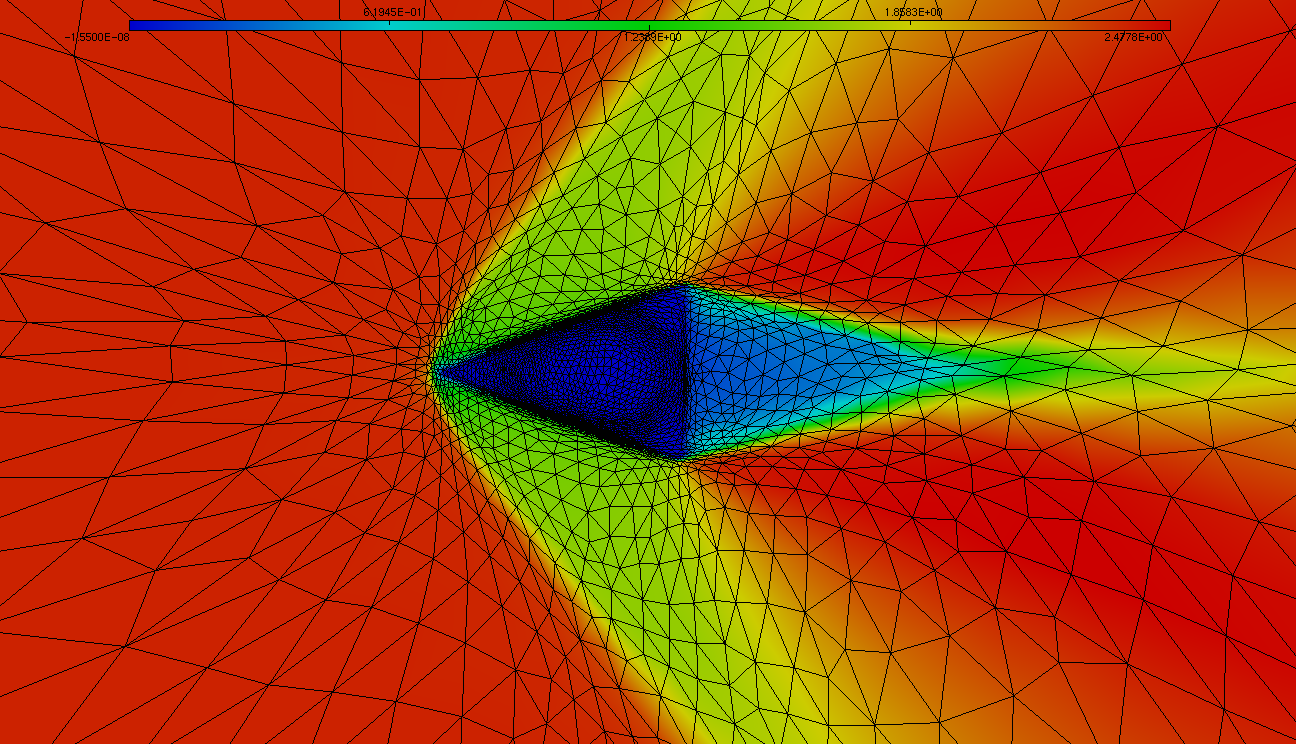
\includegraphics[scale=.15]{Bordeaux/figures/AdapPhysique/u.png}
		\captionof{subfigure}{Composant horizontale de la vitesse}
	\end{minipage}
	\hfill
	\begin{minipage}[t]{.5\linewidth}
		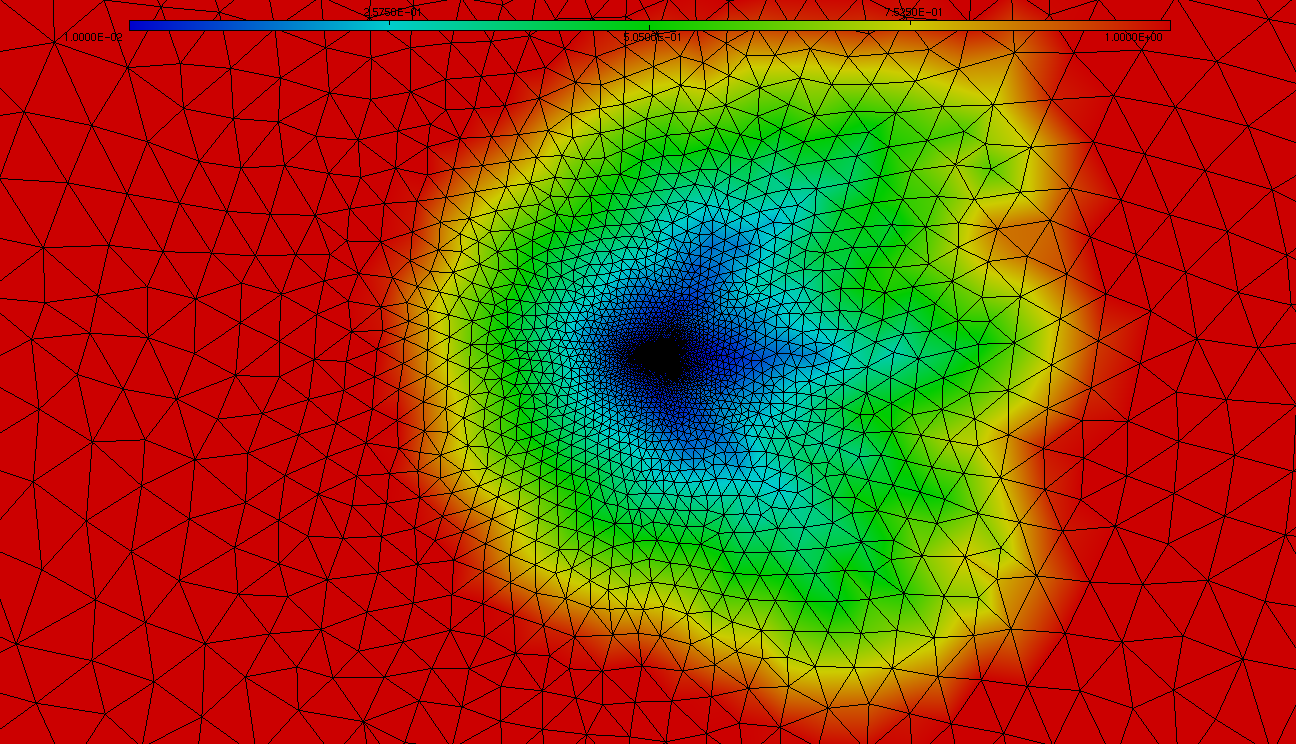
\includegraphics[scale=.15]{Bordeaux/figures/AdapPhysique/met.png}
		\captionof{subfigure}{Tailles calculées à partir de la métrique associée}
	\end{minipage}	
	\captionof{figure}{Écoulement autour d'un triangle - calcul des tailles désirées à partir d'une variable physique \label{fig:metPhys}}
\endgroup

\indent

\indent Aussi comme dans le cas de l'adaptation à des fonctions Level Set, on a plutôt utilisé dans l'adaptation physique le calcul des tailles désirées pour déterminer le mouvement des points du maillage. Les raisons sont les mêmes que celles présentées précédemment : du point de vue de l'utilisateur final, cette procédure, qui demande la définition des seuils pour la taille désirée, a un sens physique intuitif, étant ainsi plus accessible.

\subsection{Couplage entre adaptation Level Set et adaptation physique}

\indent L'objectif principal de l'ensemble du travail réalisée dans ce projet est l'application du modèle et de la bibliothèque développés à la résolution de problèmes de la mécanique de fluides, afin d'améliorer la précision des résultats. Ainsi, un bon maillage serait adapté au même temps à la surface de l'objet dans le domaine et au profil de la variable physique calculée (la vitesse, par exemple), et par conséquent les deux types de adaptation présentées ci-dessus doivent être considérées.

\indent Pour coupler les deux adaptations, on intersecte ses respectives métriques: en notant \(h_i^{LS}\) et \(h_i^{phys}\) la taille calculée pour le noeud \(i\) à partir des métriques, respectivement, de la fonction Level Set et de la variable physique (avant le lissage), on choisit le taille

\begin{equation*}
	h_i = \min(h_i^{LS},h_i^{phys})
\end{equation*}

\indent Ensuite, on applique le même lissage avec une gradation de 10\%.

\indent Pour le couplage des deux adaptations, on propose la procédure itérative suivante :  

\begin{enumerate}
	\item Calcul de la métrique associée à la fonction Level Set;
	\item Adaptation du maillage à cette métrique;
	\item \label{item:resolution} Résolution du problème physique sur le maillage adapté;
	\item Calcul de la métrique associée à la variable physique et intersection avec la métrique de la fonction Level Set;
	\item Adaptation du maillage à cette métrique, en partant du dernier maillage obtenu, mais toujours avec le même maillage de référence (le maillage de départ, non adapté);
	\item Retour au pas \ref{item:resolution}.
\end{enumerate}

\subsection{Résultats}

\indent La procédure décrite ci-dessus a été utilisé dans la résolution d'un flot supersonique 2D autour d'un triangle, avec une méthode de distribution de résidus appliquée aux équations de Navier Stokes pénalisées. Ce cas test est présenté et résolu dans \cite{leo}, dont les paramètres de l'écoulement sont les mêmes utilisés ici.

\indent Étant le modèle pénalisé, le triangle n'est pas discrétisée dans le domaine, ce qui signifie qu'il y a des mailles à son intérieur. En effet, le terme de pénalisation est appliqué exactement aux noeuds à l'intérieur de l'objet, identifiés par la signe de la fonction Level Set. Ainsi, la première adaptation de notre procédure (adaptation à la ligne de niveau 0 de la fonction Level Set) est de grande importance pour la représentation de la surface et la résolution précise des équations dans ses voisinages.

\indent La solution physique utilisée pour les adaptations suivantes est la composante horizontale de la vitesse. 

\indent Les tests ont été réalisées avec l'objectif de vérifier l'évolution de la qualité du résultat dans chaque itération de la procédure. Cette vérification a été faite de façon qualitative et quantitative. Pour la première, on a regardé par exemple la régularité du profil de la vitesse et de ses lignes de niveau et la résolution autour des coins du triangle. Pour la deuxième, on a adopté le même critère utilisé par \cite{leo}, en calculant l'angle entre le choc et l'axe \(y=0\), en utilisant un point du choc proche à cet axe, et identifiée par la proximité des lignes de niveau de la vitesse. La résolution analytique du problème fournit un angle \(\beta=53.33^o\), qu'on a utilisé pour la comparaison.

\indent Le résultat présenté dans les figures \ref{fig:adapPhysDoms} à \ref{fig:adapPhysPlotB} a été fait sur un domaine circulaire, de rayon vingt fois plus grand que la taille du triangle, afin de représenter un domaine infini, qui minimise l'influence des bords. Afin d'éviter un nombre trop grand de points, mais encore avec un bon raffinement dans les régions les plus proches des bords pour bien capturer le choc, les tailles des éléments ont été définies en fonction de la distance au centre du domaine, augmentant linéairement entre 0.002 et 1. Le résultat est un maillage avec 12664 noeuds et 25200 éléments.

\indent

\begingroup
	\begin{minipage}[t]{.5\linewidth}
		\centering
		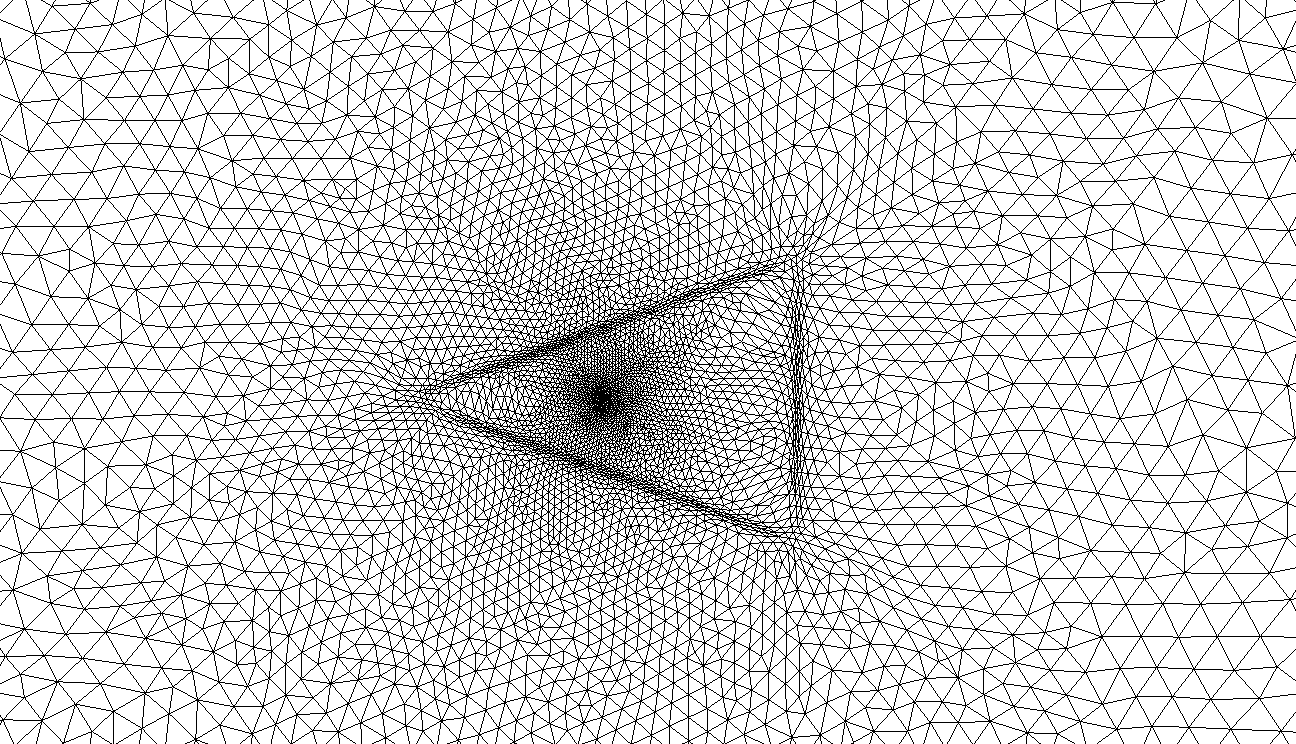
\includegraphics[scale=.15]{Bordeaux/figures/AdapPhysique/dom4bI0.png}
		\captionof{subfigure}{Première adaptation}
	\end{minipage}
	\hfill
	\begin{minipage}[t]{.5\linewidth}
		\centering
		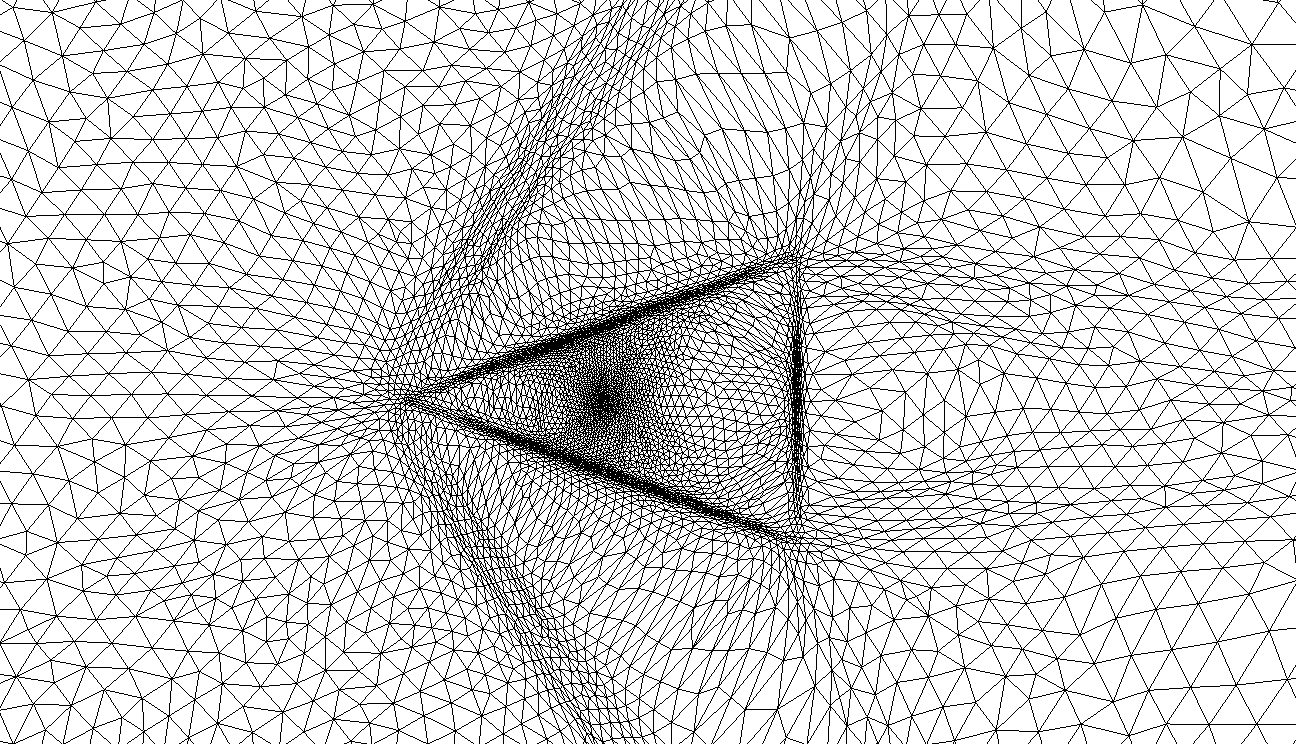
\includegraphics[scale=.15]{Bordeaux/figures/AdapPhysique/dom4bI1.png}
		\captionof{subfigure}{Deuxième adaptation}
	\end{minipage}
	\begin{minipage}[t]{1.\linewidth}
		\centering
		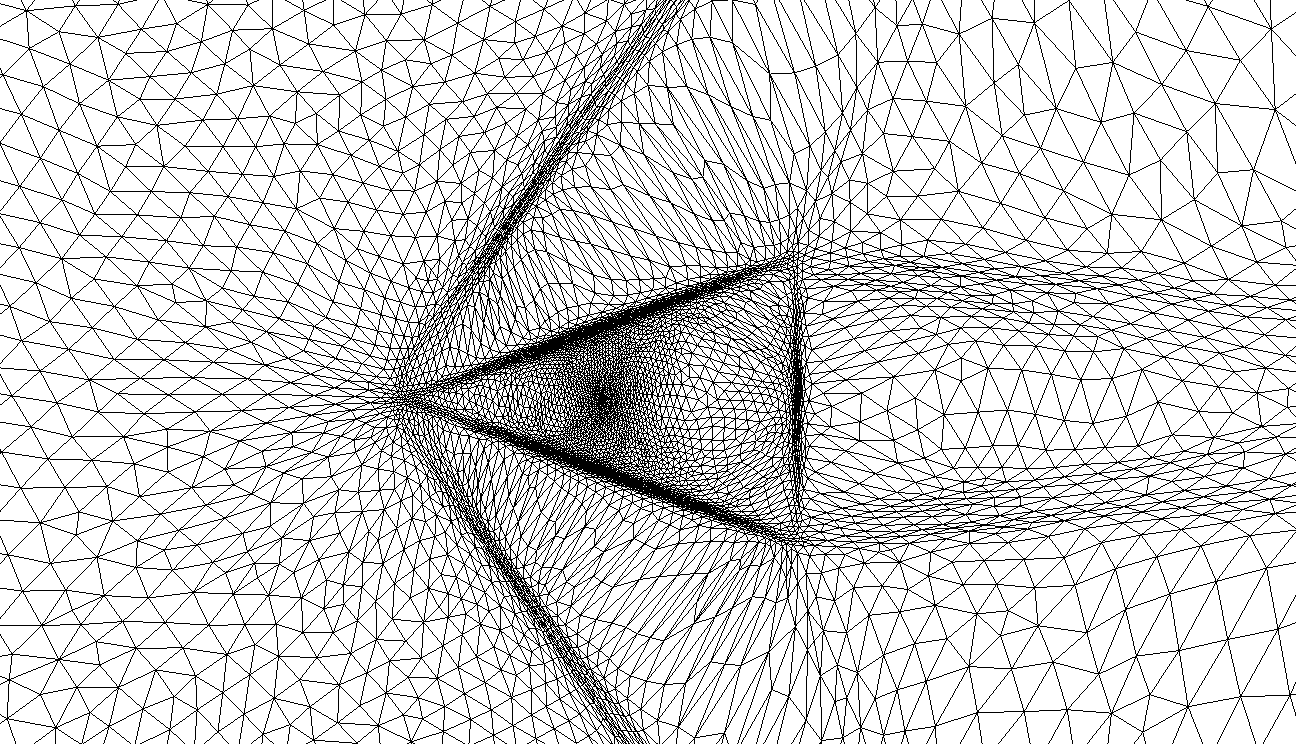
\includegraphics[scale=.15]{Bordeaux/figures/AdapPhysique/dom4bI2.png}
		\captionof{subfigure}{Troisième adaptation}
	\end{minipage}
	\captionof{figure}{Séquence de maillages adaptés obtenus \label{fig:adapPhysDoms}}
\endgroup

\newpage

\begingroup
	\begin{minipage}[t]{.5\linewidth}
		\centering
		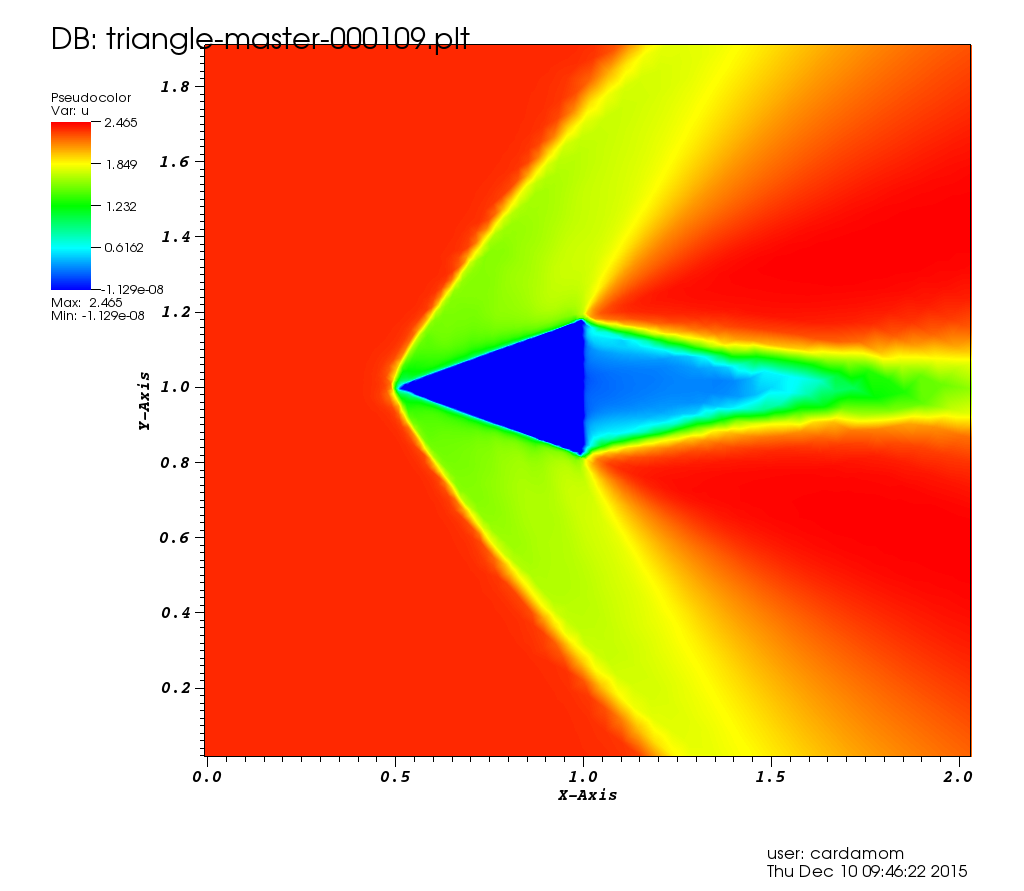
\includegraphics[scale=.2]{Bordeaux/figures/AdapPhysique/Plot4bI0A.png}
		\captionof{subfigure}{Première résolution}
	\end{minipage}
	\hfill
	\begin{minipage}[t]{.5\linewidth}
		\centering
		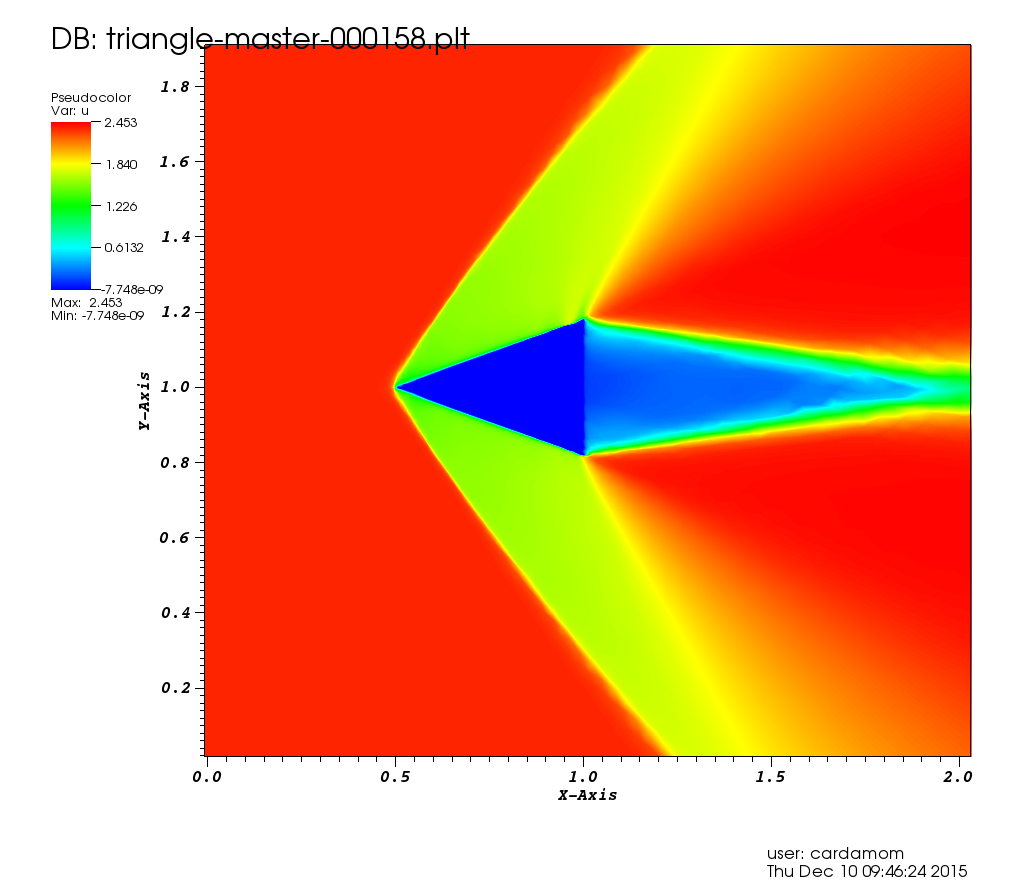
\includegraphics[scale=.2]{Bordeaux/figures/AdapPhysique/Plot4bI1A.png}
		\captionof{subfigure}{Deuxième résolution}
	\end{minipage}
	\begin{minipage}[t]{1.\linewidth}
		\centering
		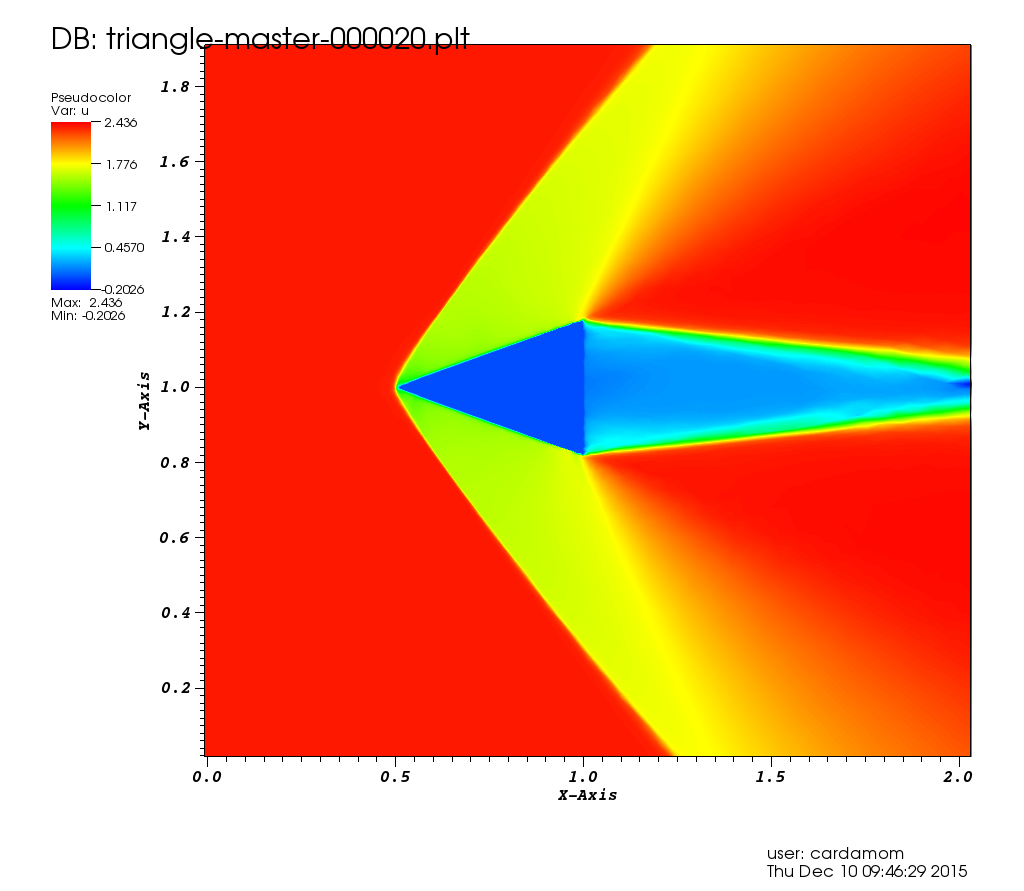
\includegraphics[scale=.2]{Bordeaux/figures/AdapPhysique/Plot4bI2A.png}
		\captionof{subfigure}{Troisième résolution}
	\end{minipage}
	\captionof{figure}{Composante horizontale de la vitesse \label{fig:adapPhysPlotA}}
\endgroup

\newpage

\begingroup
	\begin{minipage}[t]{.5\linewidth}
		\centering
		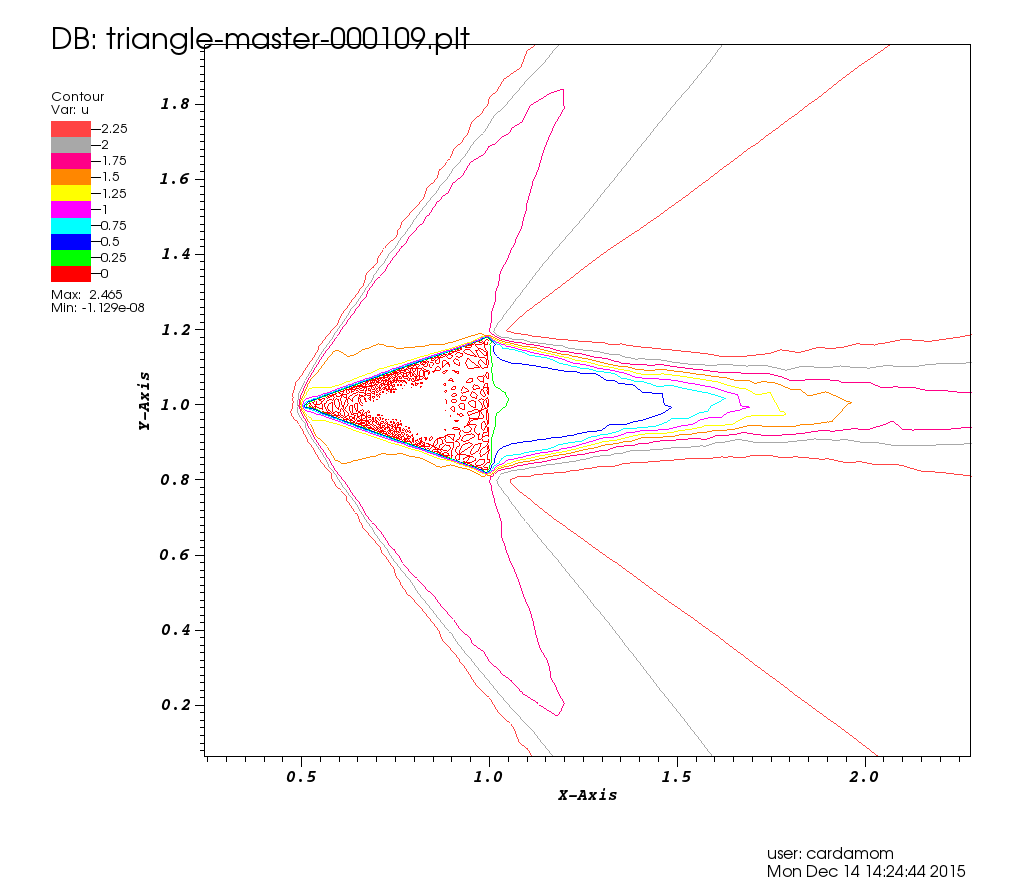
\includegraphics[scale=.2]{Bordeaux/figures/AdapPhysique/Contour4bI0.png}
		\captionof{subfigure}{Première résolution}
	\end{minipage}
	\hfill
	\begin{minipage}[t]{.5\linewidth}
		\centering
		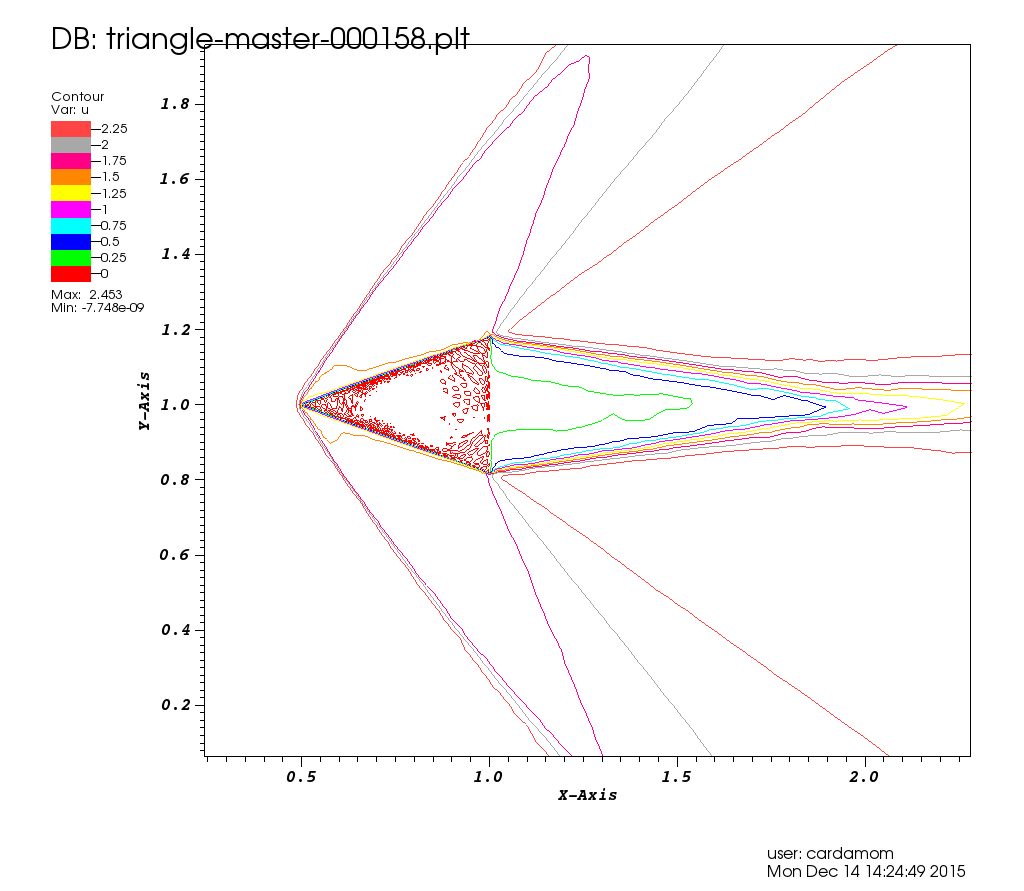
\includegraphics[scale=.2]{Bordeaux/figures/AdapPhysique/Contour4bI1.png}
		\captionof{subfigure}{Deuxième résolution}
	\end{minipage}
	\begin{minipage}[t]{1.\linewidth}
		\centering
		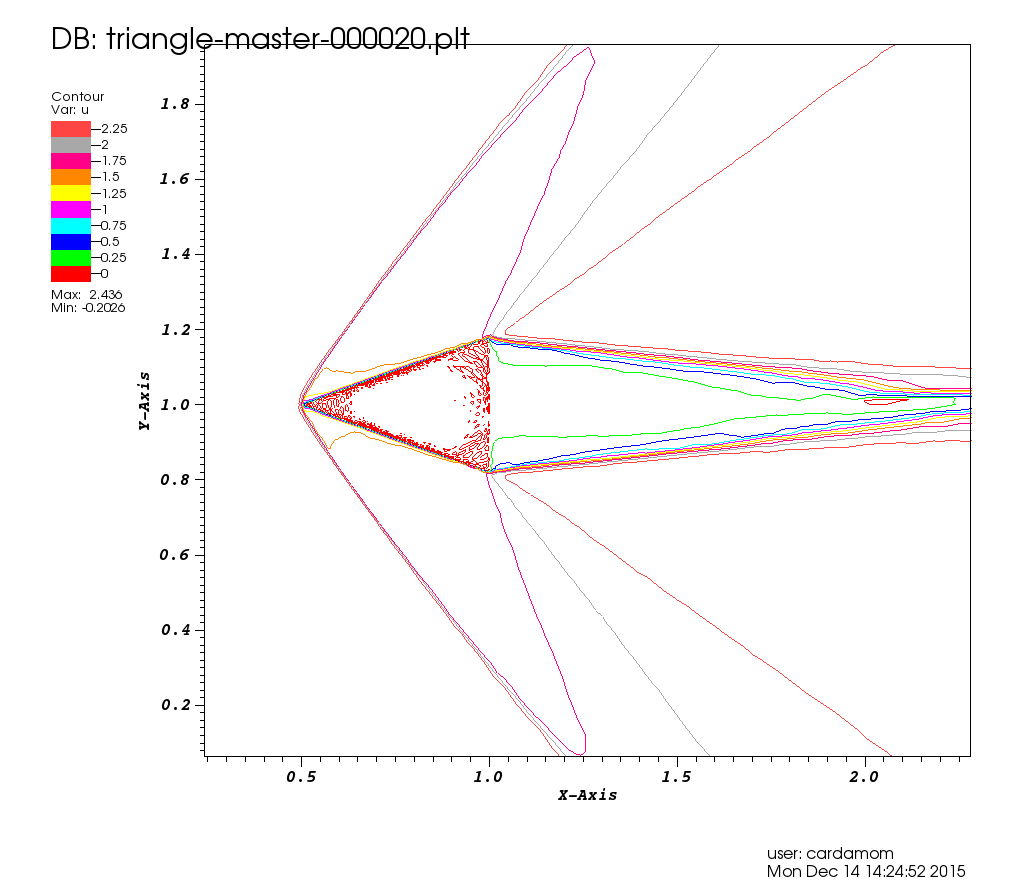
\includegraphics[scale=.2]{Bordeaux/figures/AdapPhysique/Contour4bI2.png}
		\captionof{subfigure}{Troisième résolution}
	\end{minipage}
	\captionof{figure}{Lignes de niveau de la composante horizontale de la vitesse \label{fig:adapPhysContour}}
\endgroup

\newpage

\begingroup
	\begin{minipage}[t]{.5\linewidth}
		\centering
		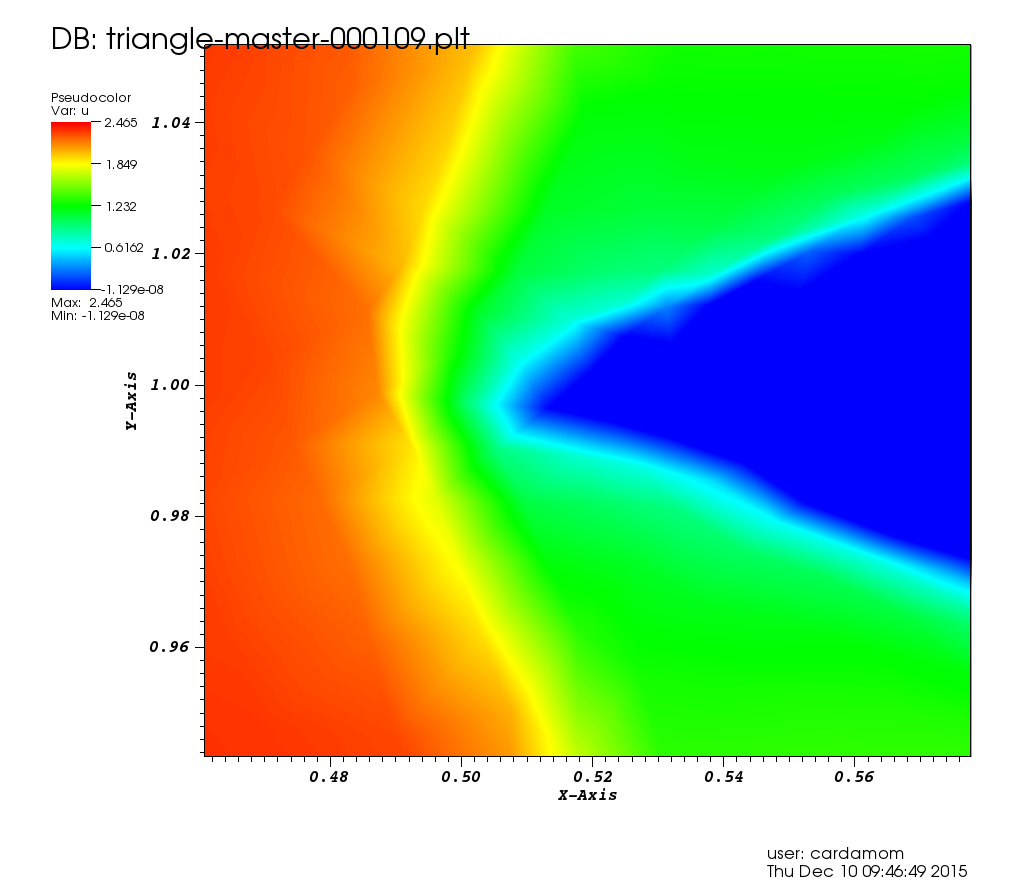
\includegraphics[scale=.2]{Bordeaux/figures/AdapPhysique/Plot4bI0B.png}
		\captionof{subfigure}{Première résolution}
	\end{minipage}
	\begin{minipage}[t]{.5\linewidth}
		\centering
		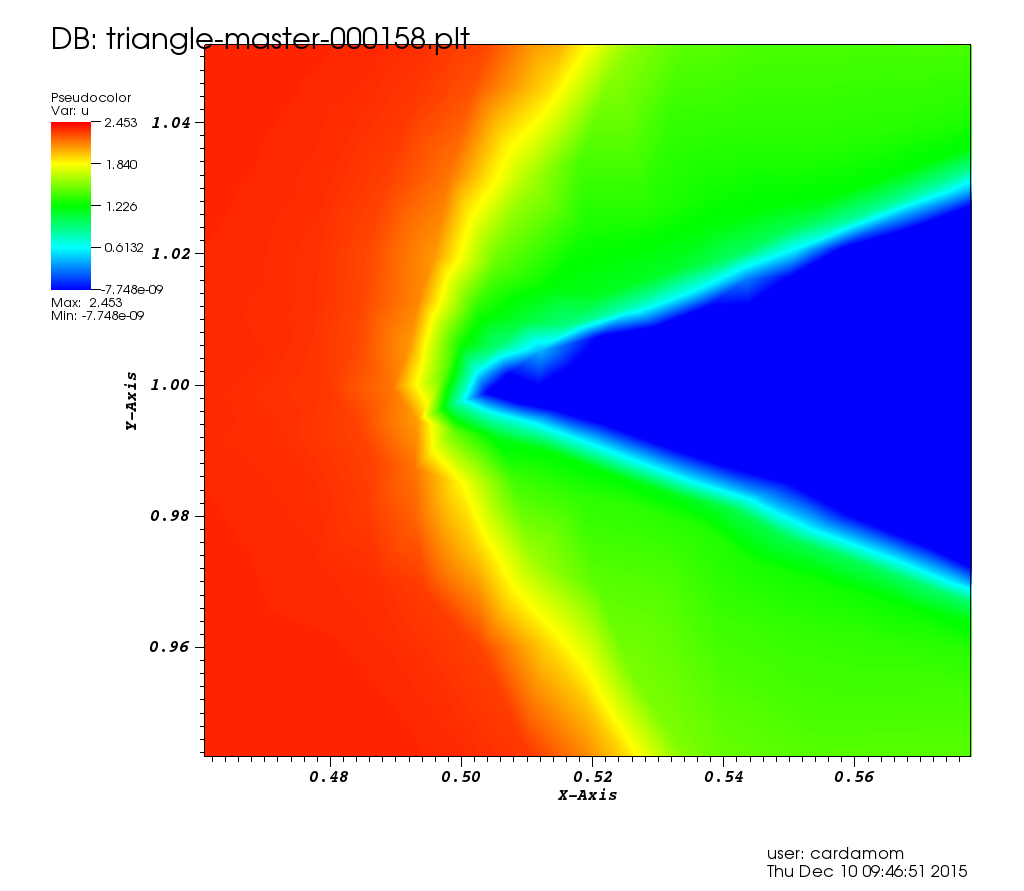
\includegraphics[scale=.2]{Bordeaux/figures/AdapPhysique/Plot4bI1B.png}
		\captionof{subfigure}{Deuxième résolution}
	\end{minipage}
	\begin{minipage}[t]{1.\linewidth}
		\centering
		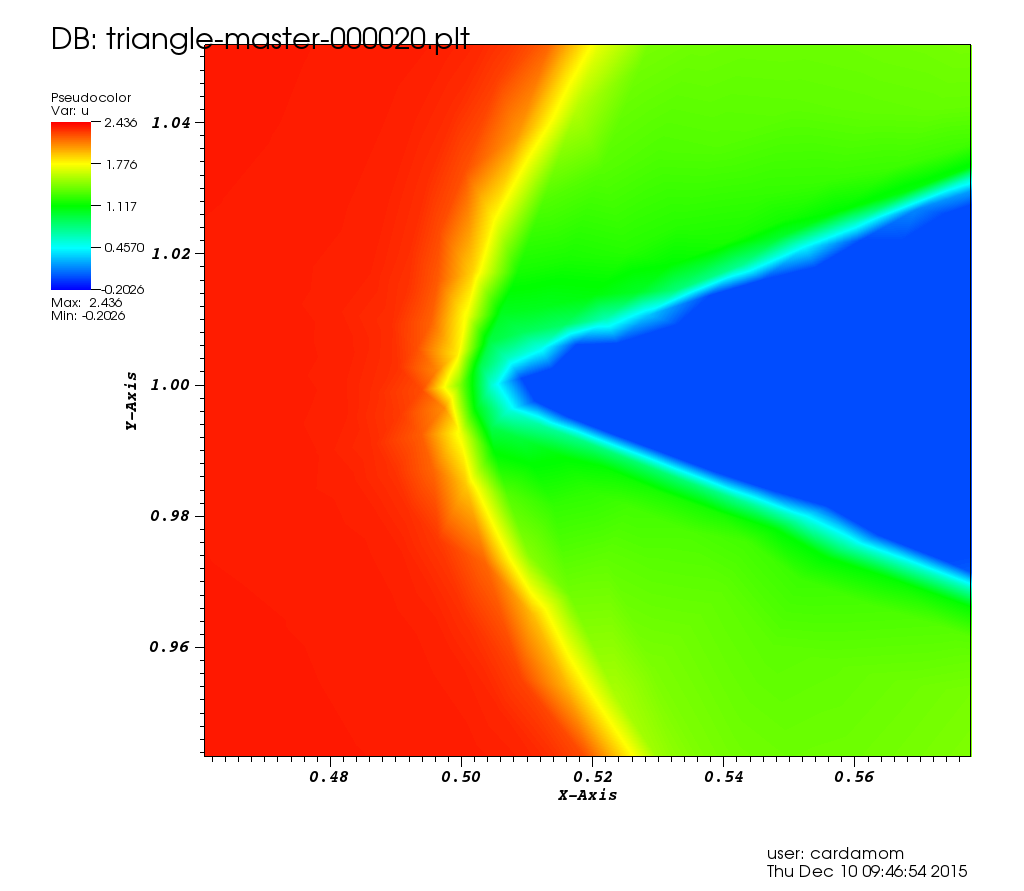
\includegraphics[scale=.2]{Bordeaux/figures/AdapPhysique/Plot4bI2B.png}
		\captionof{subfigure}{Troisième résolution}
	\end{minipage}
	\captionof{figure}{Détail - Composante horizontale de la vitesse \label{fig:adapPhysPlotB}}
\endgroup

\indent

\indent L'angle \(\beta\) a évolué selon les valeurs présentées dans le tableau \ref{tab:beta}

\begin{table}[!ht]
	\centering
	\begin{tabular}{c|c}
		Résolution & \(\beta\) \\
		\hline
		1 & \(55.68^\circ\) \\
		2 & \(53.92^\circ\) \\
		3 & \(53.01^\circ\) \\
	\end{tabular}
	\caption{Angle entre le choc et l'axe \(y=0\) \label{tab:beta}}
\end{table}

\indent Ces résultats montrent que la procédure proposée permet en effet d'améliorer la résolution du problème physique : à chaque itération, le champ de vitesse calculée devient mieux définie, avec des lignes de niveau plus régulières, et l'angle entre le choc et l'axe \(y=0\) s'approche de la valeur analytique. Néanmoins, quelques difficultés sont encore présentes dans las tests réalisées, notamment la génération de maillages permettant un calcul stable (considérant les fortes discontinuités qui caractérisent ce cas test) et le fait que, comme montre la figure \ref{fig:adapPhysPlotB}, le choc n'est pas attaché au triangle, au contraire du résultat théorique, ce qui s'explique par les limitations du raffinement du maillage.
  
\section{Adaptation à un cas non stationnaire}
\label{sec:nonstat}

\indent Les résultats présentés dans les sections précédentes se référent à des cas stationnaires, avec les surfaces fixes, mais une situation qu'on veut considérer aussi  est celle où les objets bougent. Dans ce cas, il faut à chaque pas de temps actualiser la fonction Level Set et adapter le maillage autour de la nouvelle position de la surface. La procédure adoptée est la suivante : 

\begin{enumerate}
	\item Pour tout noeud du maillage, calculer la fonction Level Set par rapport à la position actuelle de l'objet, et la fonction \(u\) à adapter (equation \eqref{eq:atan});
	\item Adapter le maillage à la fonction \(u\);
	\item Faire bouger la surface de l'objet (indépendamment de la position des noeuds)
\end{enumerate}

\indent L'objectif de cette procédure est de faire chaque adaptation à partir du dernier maillage adapté, au lieu de partir du maillage non adapté à chaque pas du mouvement. Ainsi, on peut éviter de garder en mémoire toute la structure du maillage de référence et du maillage adapté. Il faut pourtant garder au moins les aires et les vecteurs normaux du maillage, parce que, en raison du modèle adopté, toutes les adaptations doivent utiliser le même maillage de référence.

\indent Les figures \ref{fig:circleLSAdv} et \ref{fig:nacaLSAdv} présentent deux exemples de cette procédure, le premier pour l'advection d'un cercle et le deuxième pour l'oscillation de l'aile Naca. Les mouvements on été discrétisées en 20 pas de temps, et chaque itération a été réalisée avec 20 ou 30 itérations, respectivement.

\indent On peut observer qu'on obtient à chaque pas de temps une bonne adaptation à la position actuelle de la fonction Level Set, mais que les positions précédentes ne sont pas complètement ``désadaptées", même que son trace soit faible. En effet, les tests montrent que le passage d'une adaptation à la prochaine se fait de deux manières (en dépendant de la position des points adaptés pour la position précédente) : soit par le mouvement des points d'une région adaptée à l'autre (ce qui est possible quand le point est relativement proche de la nouvelle position de l'objet), soit par le ``dérafinement" d'une région (ce qui est le cas des points en amont du mouvement de l'objet). On a observé que le deuxième cas est plus lente que le premier, et ainsi on aurait besoin d'un plus grand nombre d'itérations. Néanmoins, pour justifier l'application de cette procédure, il faut trouver un équilibre entre le temps d'exécution et la qualité des résultats.

\indent

\begingroup
	\begin{minipage}[t]{.5\linewidth}
		\centering
		 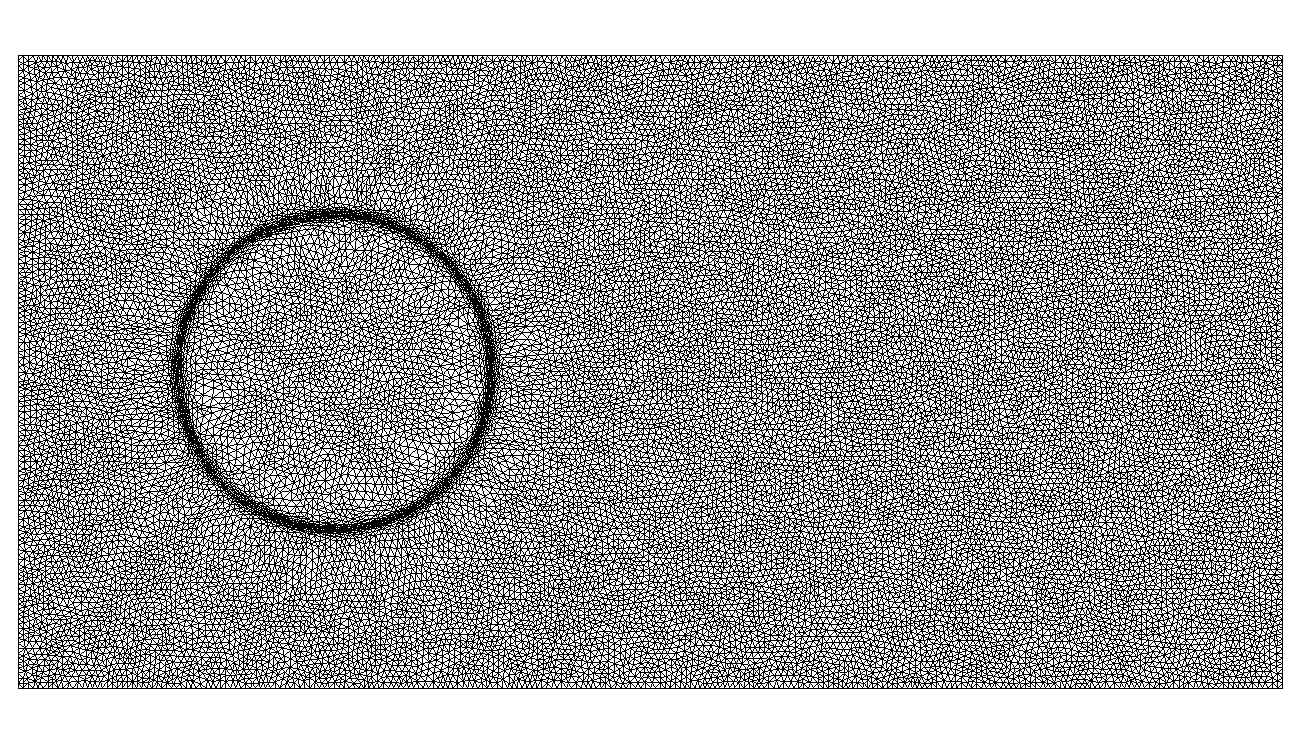
\includegraphics[scale=.15]{Bordeaux/figures/LSAdvection/CircleAdvNew0.png}
		 \captionof{subfigure}{Pas n. 0}
	\end{minipage}
	\begin{minipage}[t]{.5\linewidth}
		\centering
		 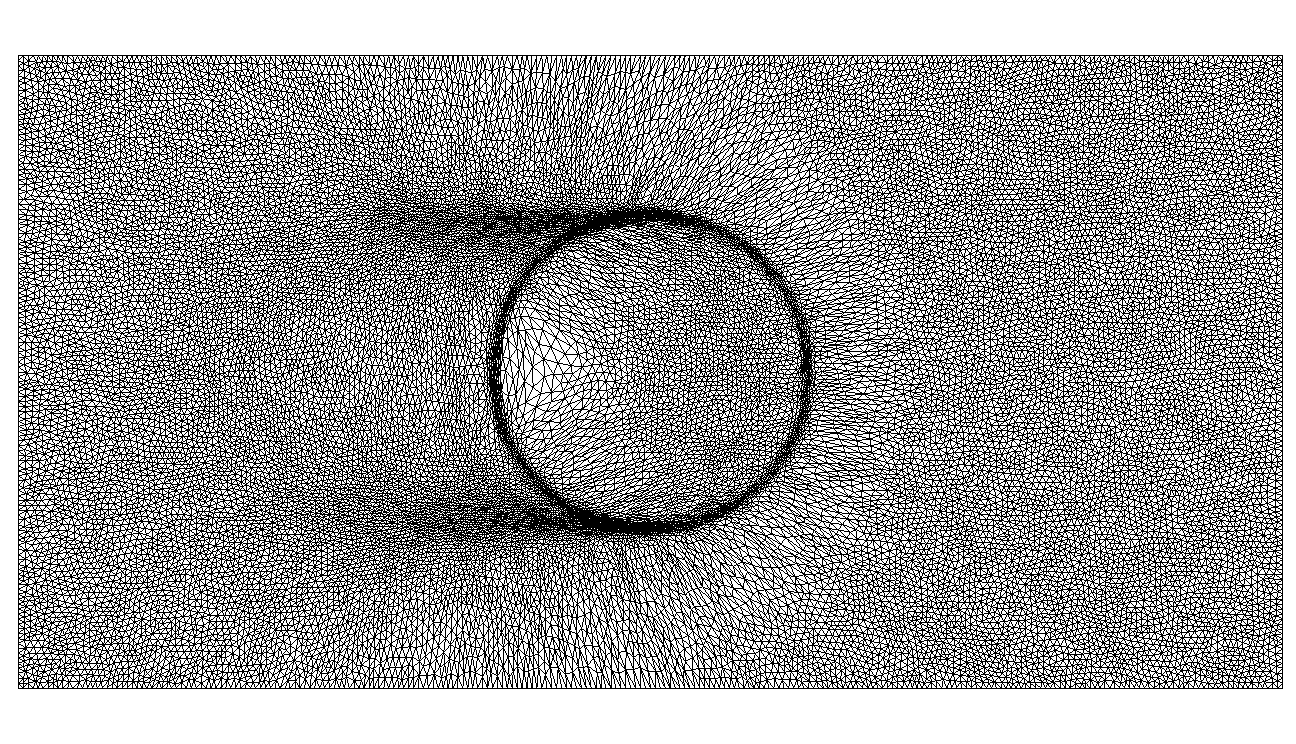
\includegraphics[scale=.15]{Bordeaux/figures/LSAdvection/CircleAdvNew10.png}
		 \captionof{subfigure}{Pas n. 10}
	\end{minipage}
	\begin{minipage}[t]{1.\linewidth}
		\centering
		 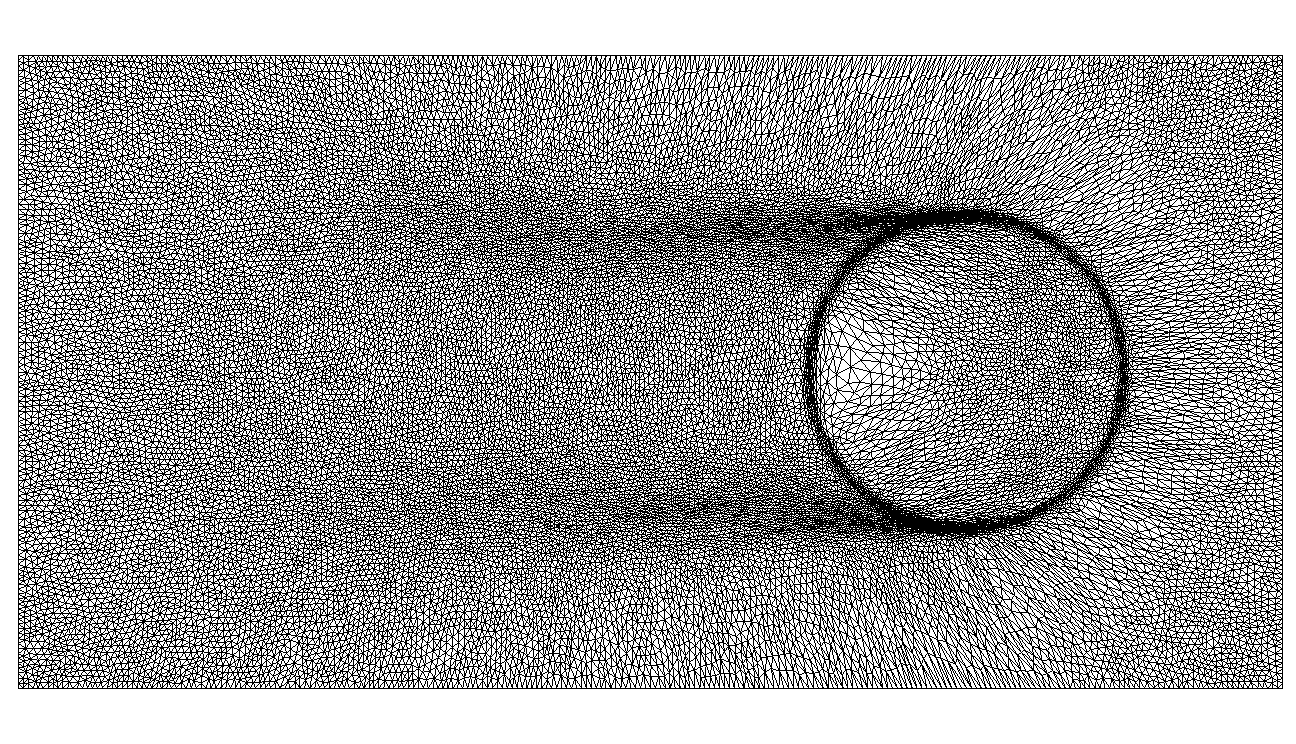
\includegraphics[scale=.15]{Bordeaux/figures/LSAdvection/CircleAdvNew20.png}
		 \captionof{subfigure}{Pas n. 20}
	\end{minipage}
	\captionof{figure}{Advection d'un cercle \label{fig:circleLSAdv}}
\endgroup

\indent

\indent

\begingroup
	\begin{minipage}[t]{.5\linewidth}
		\centering
		 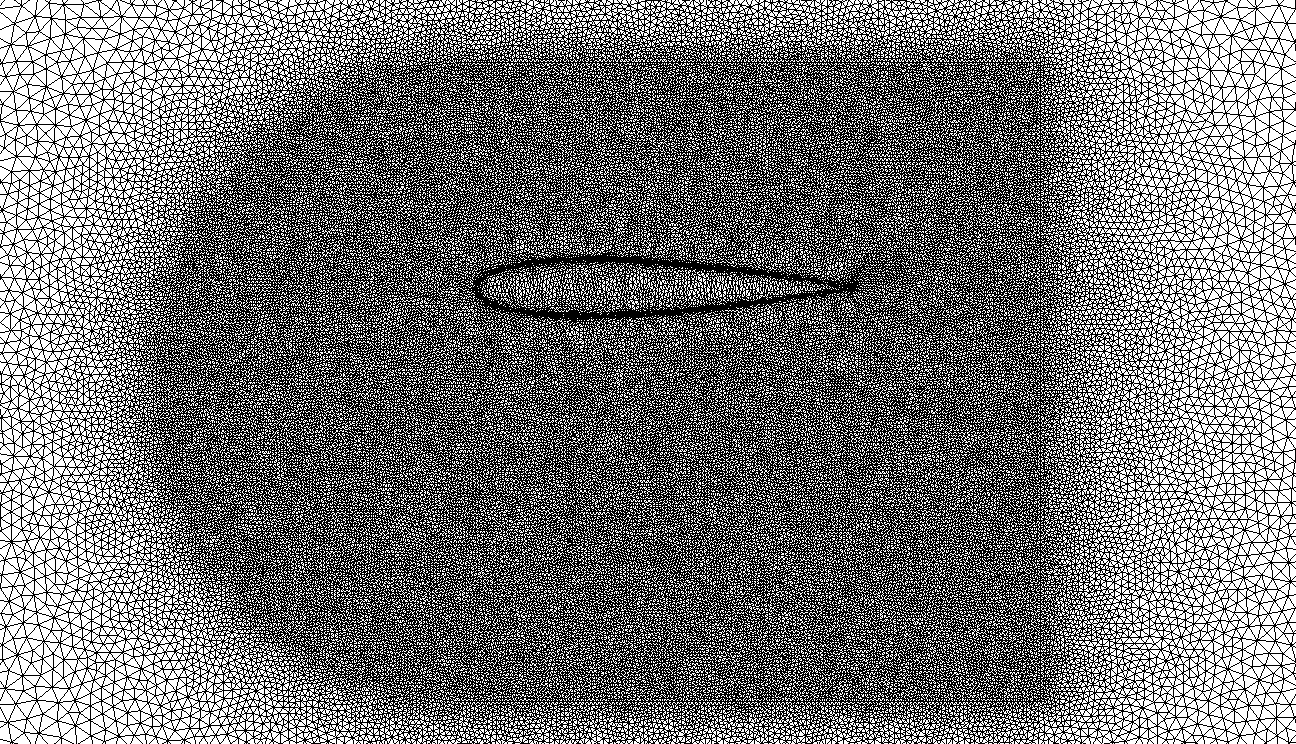
\includegraphics[scale=.15]{Bordeaux/figures/LSAdvection/NacaAdvNew0.png}
		 \captionof{subfigure}{Pas n. 0}
	\end{minipage}
	\begin{minipage}[t]{.5\linewidth}
		\centering
		 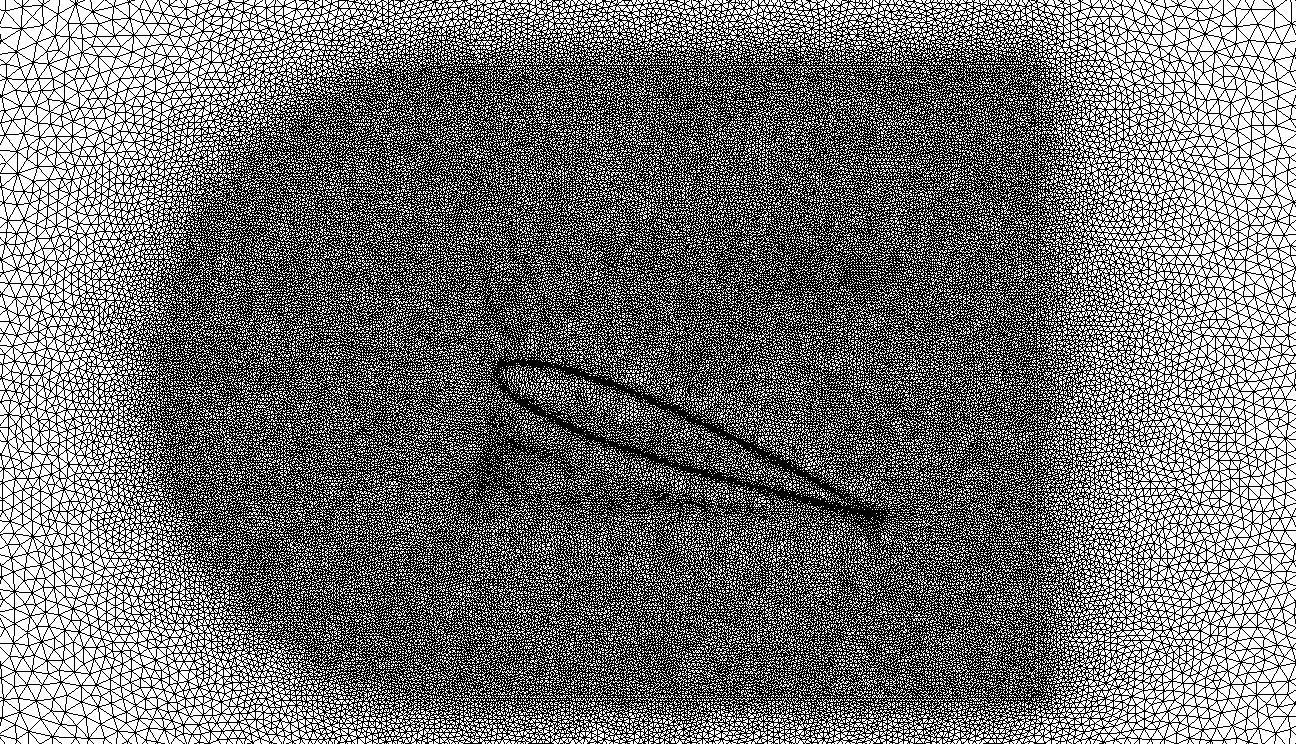
\includegraphics[scale=.15]{Bordeaux/figures/LSAdvection/NacaAdvNew10.png}
		 \captionof{subfigure}{Pas n. 10}
	\end{minipage}
	\begin{minipage}[t]{1.\linewidth}
		\centering
		 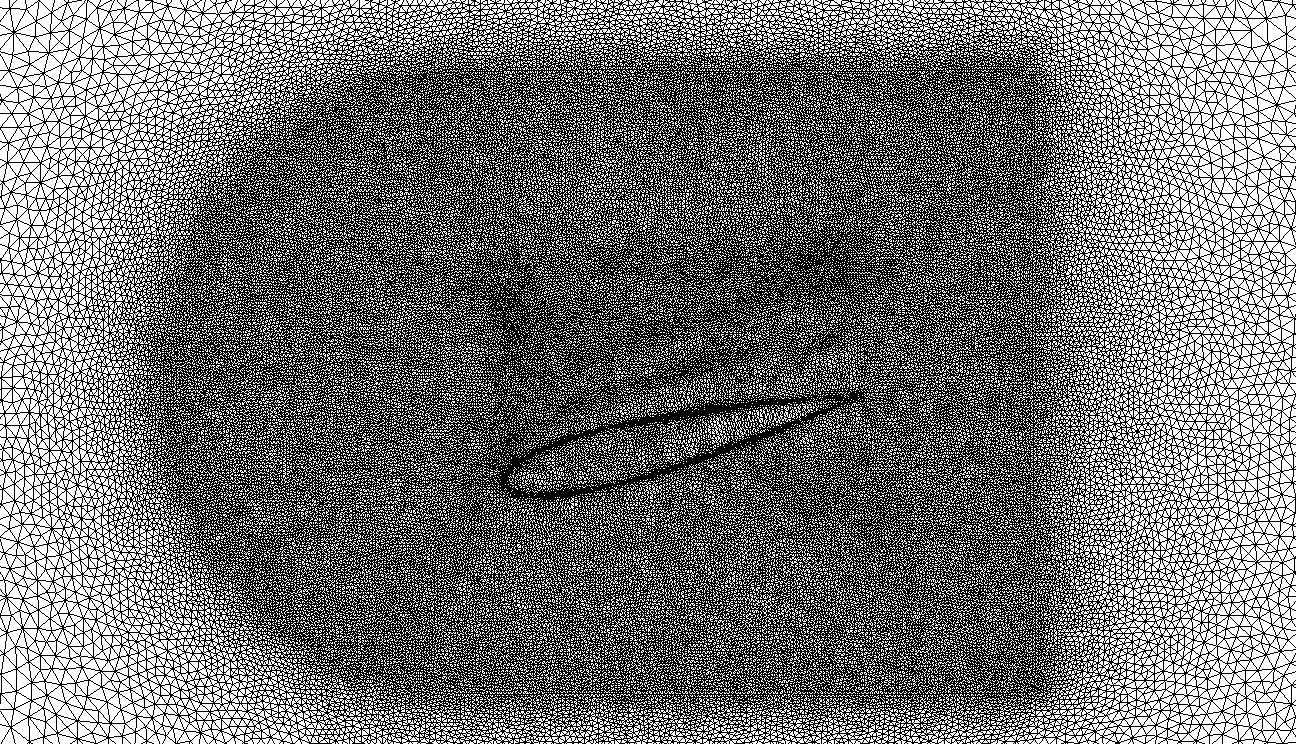
\includegraphics[scale=.15]{Bordeaux/figures/LSAdvection/NacaAdvNew20.png}
		 \captionof{subfigure}{Pas n. 20}
	\end{minipage}
	\captionof{figure}{Naca oscillant \label{fig:nacaLSAdv}}
\endgroup



%\indent L'approche qu'on a d'abord essayé, envisageant une économie de l'espace mémoire utilisé pour l'exécution du programme, était de faire l'adaptation, à chaque pas de temps, à partir du dernier maillage calculé. Néanmoins, les tests ont présenté plusieurs problèmes qui se montrent incontournables avec le modèle d'adaptation qu'on utilise, notamment : 
%
%\begin{itemize}
%	\item Le modèle ne provoque pas un "dé-raffinement" des éléments. Ainsi, dans le résultat final, on peut observer le trace de la marche de l'objet sur le maillage (figure \ref{fig:optim_bad});
%	\item Les éléments raffinés dans un certain pas de temps n'arrivent pas à bouger jusqu'à la nouvelle position, soit en raison de la très fréquente relaxation (principalement quand on discrétise le mouvement de la surface avec un petit pas de temps, car les adaptations successives sont faites presque sur le même endroit), soit parce qu'il sont très éloignés de la nouvelle position (principalement quand le pas de temps est trop grand).
%\end{itemize}
%
%	\begin{figure} [!ht]
%	  \begin{subfigure}{.5\linewidth}
%	    \centering
%	    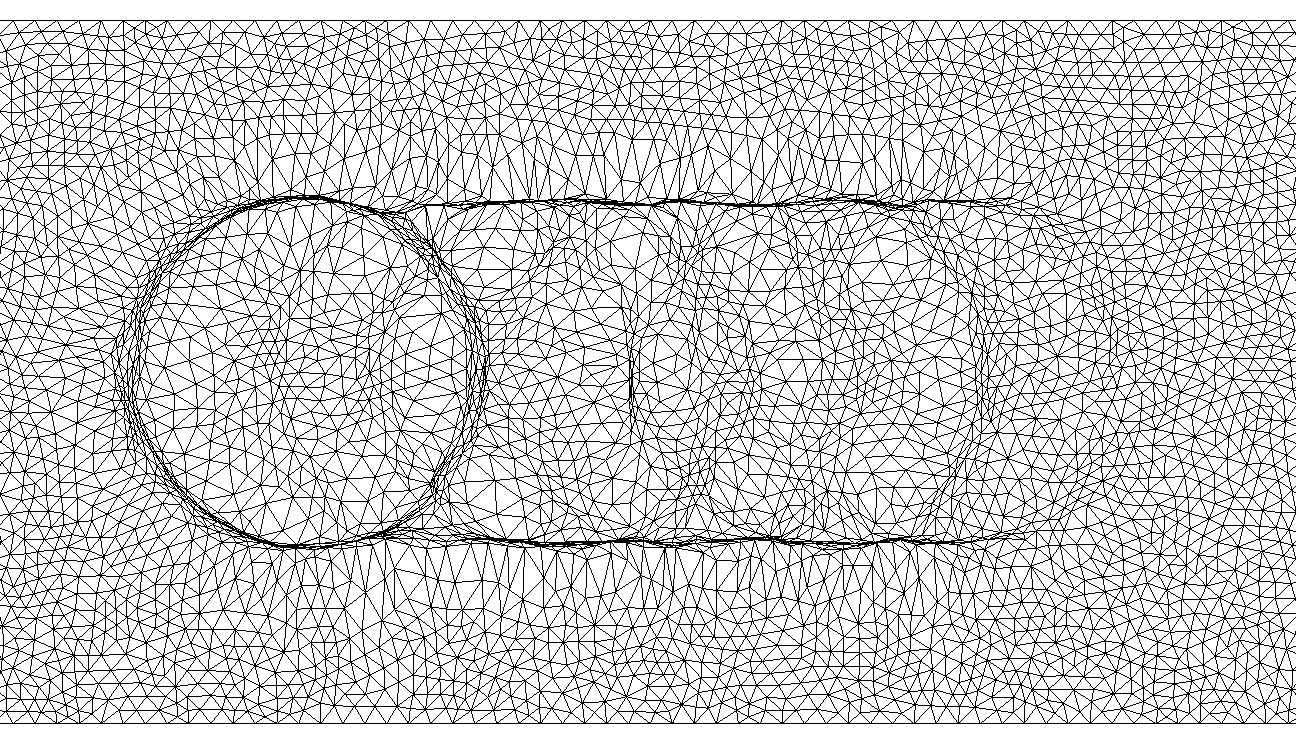
\includegraphics[scale=.12]{figures/optim_bad_circle.png}
%	  \end{subfigure} 
%	  \begin{subfigure}{.5\linewidth}
%	    \centering
%	    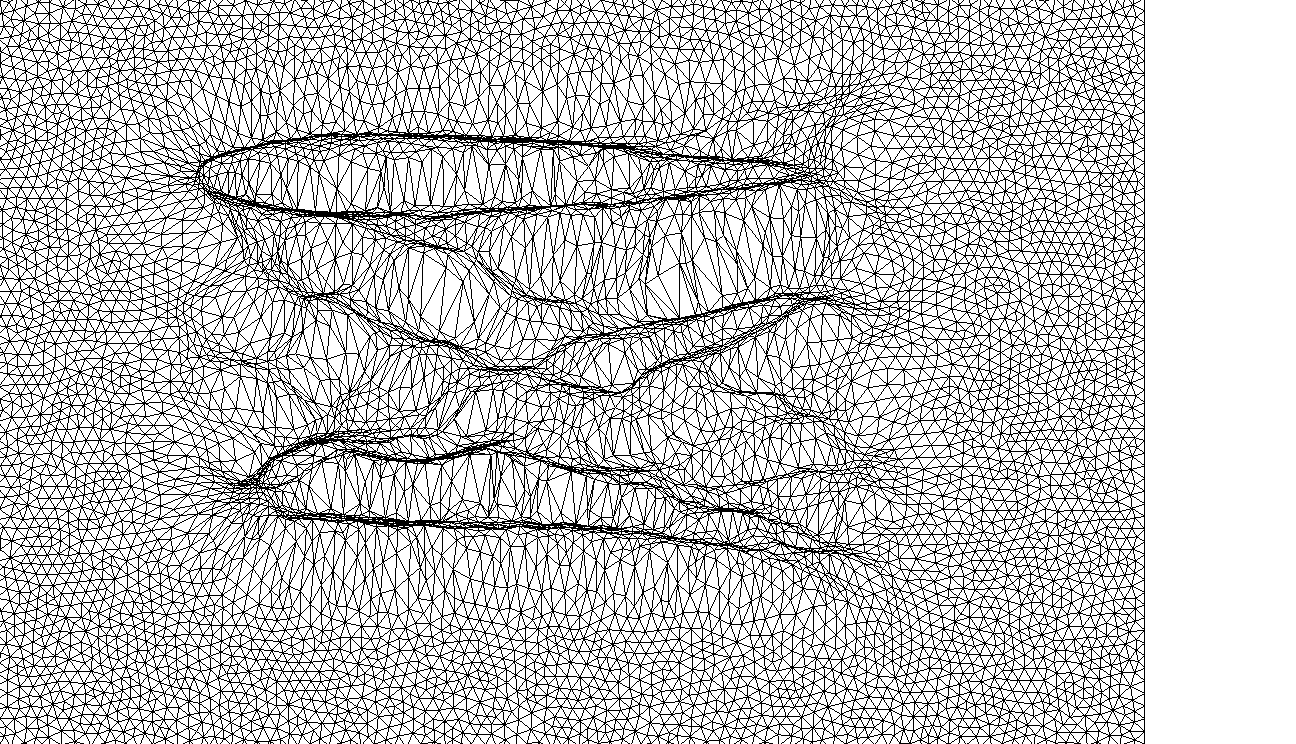
\includegraphics[scale=.12]{figures/optim_bad_naca.png}
%	  \end{subfigure}
%	  \caption{Maillages finaux des adaptions partant du maillage initial à chaque pas du mouvement de la surface \label{fig:optim_bad}}
%	\end{figure}
%
%\indent L'unique solution trouvée, ainsi, est de faire chaque adaptation en partant toujours du maillage initial. On obtient ainsi des très bons résultats, comme montrent les figures \ref{fig:optim_good_1} et \ref{fig:optim_good_2}, car les adaptations sont indépendantes, mais pour cela il faut garder le maillage initial en mémoire.
%
%	\begin{figure} [!ht]
%	  \begin{subfigure}{.5\linewidth}
%	    \centering
%	    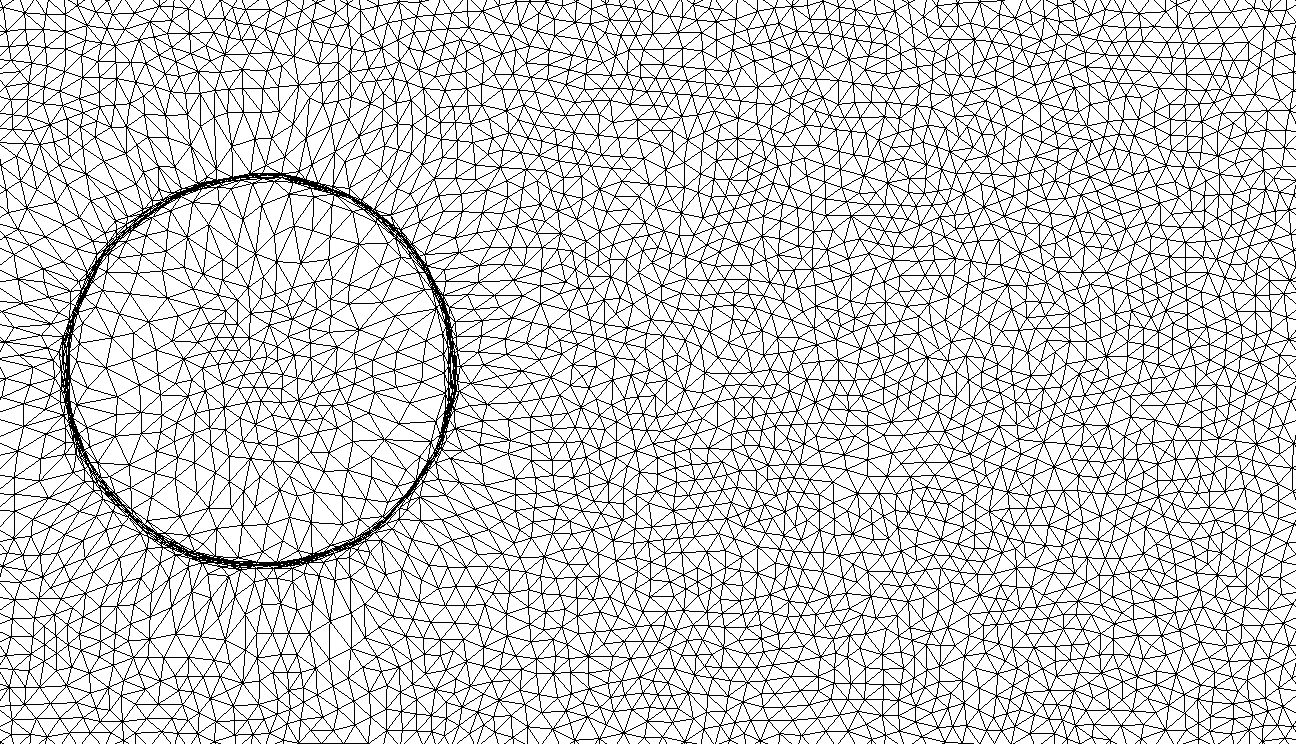
\includegraphics[scale=.12]{figures/optim_good_circle0.png}
%	  \end{subfigure} 
%	  \begin{subfigure}{.5\linewidth}
%	    \centering
%	    \includegraphics[scale=.12]{figures/optim_good_circle1.png}
%	  \end{subfigure}
%	  \begin{subfigure}{.5\linewidth}
%	    \centering
%	    \includegraphics[scale=.12]{figures/optim_good_circle2.png}
%	  \end{subfigure}
%	  \begin{subfigure}{.5\linewidth}
%	    \centering
%	    \includegraphics[scale=.12]{figures/optim_good_circle3.png}
%	  \end{subfigure} 
%	  \caption{Adaptation à un cercle advecté \label{fig:optim_good_1}}
%	\end{figure}
%	
%	\begin{figure} [!ht]
%	  \begin{subfigure}{.5\linewidth}
%	    \centering
%	    \includegraphics[scale=.12]{figures/optim_good_naca0.png}
%	  \end{subfigure} 
%	  \begin{subfigure}{.5\linewidth}
%	    \centering
%	    \includegraphics[scale=.12]{figures/optim_good_naca1.png}
%	  \end{subfigure}
%	  \caption{Adaptation au Naca oscillant \label{fig:optim_good_2}}
%	\end{figure}

  \section{Autres rapports}
\label{sec:autres}

\indent D'autres tests et résultats obtenus au long du développement du modèle et de la bibliothèque FMG peuvent être trouvés dans les rapports suivants, disposés en ordre chronologique. On put notamment observer le moment où le modèle pour le calcul de \(\omega\) a été modifié : 

\begin{itemize}
    \item \(\omega\) calculé à partir du gradient
	\begin{enumerate}
		\item Adaptation à des fonctions analytiques : rapport\_adapAnalytique.pdf, rapport\_adapCircle.pdf, rapport\_adapCircleNS.pdf
		\item Adaptation à des fonctions LevelSet : rapport\_LevelSet.pdf
		\item Calcul d'un problème physique sur des maillages adaptés : rapport\_pbFluide.pdf
		\item Adaptation physique / Level Set : rapport\_physAdapt.pdf
		\item Adaptation à une fonction Level Set advectée : rapport\_circleAdv.pdf
		\item Récapitulatif de l'adaptation Level Set : recapitulatif\_adaptLS.pdf
	\end{enumerate}
	\item \(\omega\) calculé à partir de la métrique
	\begin{enumerate}
		\item Premières approches au nouveau modèle : rapport\_metrique.pdf et rapport\_taille\_maillage.pdf
		\item Adaptation 3D : rapport\_adaptation3D.pdf
		\item Adaptation physique en utilisant la solution du problème physique calcule sur des maillages adaptés : rapport\_physAdapt.pdf
		\item Adaptation à une fonction Level Set advectée : rapport\_LSAdv.pdf
		\item Adaptation physique / Level Set : rapport\_physmetrique.pdf (texte) et GT\_en.pdf (présentation).
	\end{enumerate}	
\end{itemize}
  %\subsubsection{Algorithme d'optimisation}

\indent L'optimisation d'un certain élément \(T\) est faite selon l'algorithme \eqref{alg:optim}: 

\begin{algorithm}
	\caption{Optimisation d'un élément \(T\) \label{alg:optim}}
	\begin{algorithmic}
		\For {\(iter = 1,...,iter_{max}\)}
			\State \(continue = 0\)
			\For {\(i \in T\)}
				\State Compute $ Q_{min}^i = \min_{\To \ni i} Q_{\To} $ \Comment{ $Q$ : indicateur de qualité}
				\State $  \tilde{\vecx}_i = \frac{1}{\Nn^i} \sum\limits_{\To \ni i} { \sum\limits_{j \in \To, j\neq i}{\vecx_j}  } $ \Comment{\(\Nn^i\) : nombre de voisins de \(i\)}
			\EndFor
			\If {$ \min_{\Tt \ni i}{\frac{Q_{\Tt}}{Q_{min}^i}} < \nu $}  \Comment{$\nu \geq 1$}
				\State Relaxer
			\EndIf
			\If {$|\tilde{\vecx} - \vecx| > \epsilon $} 
				\State \(continue = 1\)
			\EndIf
			\If {$continue = 0 $}
				\State $ iter = iter_{max} $
			\EndIf
		\EndFor  
	\end{algorithmic}
\end{algorithm}
  \bibliography{bibliographie}
\end{document}